\documentclass[10pt]{beamer}
\usepackage{amsmath}
\usepackage{mathdots}
\usepackage{algorithm}
\usepackage{algorithmic}
\usepackage{tikz}

\usepackage{tikz,mathpazo}
\usetikzlibrary{shapes.geometric,arrows}
\usetikzlibrary{calc}

\usetikzlibrary{arrows}
\usetheme[progressbar=frametitle]{metropolis}
\usepackage{booktabs}
\usepackage[scale=1]{ccicons}
\usepackage{pgfplots}
\usepackage{amsmath}
\newcommand{\norm}[1]{\left\lVert#1\right\rVert}
\usepgfplotslibrary{dateplot}
\hypersetup{
    colorlinks=true,
    linkcolor=blue,
    filecolor=magenta,      
    urlcolor=cyan,
}
 
\urlstyle{same}

\usepackage{xspace}
\newcommand{\themename}{\textbf{\textsc{metropolis}}\xspace}

\title{A Fault Detection Method Based on SVM Technique with $T^2$-Statistic and Riemannian Metric}
%\subtitle{going beyond IF and Scopus index (v2.0)}
\author{Zhongcheng Dai  \\
 Supervisor: \\
 Prof. Dr. Ing. Steven Ding\\
Dr. Ing. Chris Louen 
}
 \date{12.12.2019}
\institute{Automatic Control and Complex Systems}
\titlegraphic{\hfill
\includegraphics[height=1cm]{logo_ITB}}
\begin{document}
\maketitle
\begin{frame}{contents}
  \setbeamertemplate{section in toc}[sections numbered]
  \tableofcontents[hideallsubsections]
\end{frame}
\section{Introduction}
\begin{frame}{Background}
 A brief summary of the traditional method:
      \begin{itemize}
      \item \textcolor{blue}{S1}: collect sufficient fault-free data
      \item \textcolor{blue}{S2}: offline training and determine the threshold
      \item \textcolor{blue}{S3}: online monitoring  % use the threshold to check the new data
 	 \end{itemize}  
 Detection logic:
 \begin{equation}\nonumber
 \begin{aligned}
     &J > J_{th} \quad faulty \\
     &J \leq J_{th} \quad fault-free \\
     \end{aligned}
 \end{equation}
\end{frame}
\begin{frame}{Background}
 \begin{exampleblock}{Merits of $T^2$-statistic}
	\begin{itemize}
    \item The detection performance for additive faults is satisfactory
    \item Low computational cost(threshold and online monitoring)
    \end{itemize}
    \end{exampleblock}
    \begin{exampleblock}{Drawbacks of $T^2$-statistic}
      \begin{itemize}
      \item The detection performance for multiplicative faults is unqualified
 	 \end{itemize}  
 	 \end{exampleblock}
 	   \begin{exampleblock}{Merits of Riemannian distance}
      \begin{itemize}
      \item No assumption of the distribution
      \item It can detect changes in the variance
 	 \end{itemize}  
 	 \end{exampleblock}
\end{frame}

\begin{frame}

 \begin{columns}
             \begin{column}{0.7\textwidth}
     \begin{exampleblock}{Objective}
      \begin{itemize}
      \item Eliminate the shortcomings of traditional method
      \item Enhance the fault detection performance
 	 \end{itemize}  
 	 \end{exampleblock}
 \begin{exampleblock}{Solution}
      \begin{itemize}
      \item Combine  $T^2$-statistic and Riemannian metric with Support Vector Machine:
       \begin{itemize}
         \item  Extract the feature data as the training data set
          \item Find the hyperplane as threshold
          \end{itemize}
 	 	 \end{itemize}  
 	 \end{exampleblock}   
           \end{column}
        \begin{column}{0.3\textwidth}  %%<--- here
        \begin{figure}
            \centering
            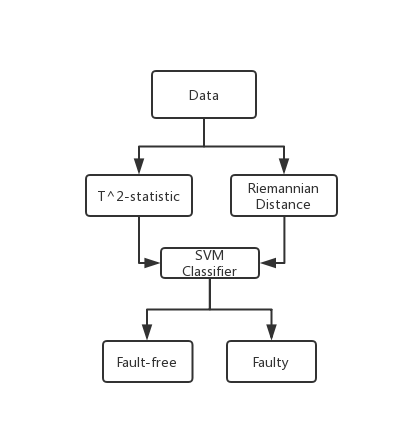
\includegraphics[width=4cm]{fig/process.png}
        \end{figure}
  
        \end{column}
    \end{columns}

\end{frame}
\section{Building monitoring index}
\begin{frame}{Data}
The data $y_{obs}(i)$ is given, where $i = 1 \dots n_1 \dots N$.
The data set $y = [y_{obs}(1) \dots y_{obs}(N)]$.
\begin{equation}
    y_{obs}(i)= 
    \begin{pmatrix}
        y_{obs,1}(i) \\
        y_{obs,2}(i) \\
       \vdots  \\
        y_{obs,m}(i) \\ 
    \end{pmatrix}
\end{equation}
Where $\textbf{m}$ is the dimension of the output data.% it is also called "degrees of freedom" in $T^2$ distribution.
\par
\end{frame}
\begin{frame}{Building monitoring index with $T^2$-statistic}
    \begin{columns}
        \begin{column}{0.5\textwidth}
            the steps: %of $T^2$-statistic:
      \begin{itemize}
      \item \textcolor{blue}{S1}: computing the mean \\
      \item \textcolor{blue}{S2}: computing the variance
      \item \textcolor{blue}{S3}: normalizing the data
      \item \textcolor{blue}{S4}: computing the  covariance
      \item \textcolor{blue}{S5}: computing the value of evaluation function
 	 \end{itemize}  
        \end{column}
        \begin{column}{0.5\textwidth}  %%<--- here
      \begin{equation} \nonumber
               \begin{aligned}
                  & E \approx \frac{1}{n_1}\sum_{i=1}^{n_1}y_{obs}(i) \\
                  & \sigma_j^2 \approx \frac{1}{n_1-1}\sum_{i=1}^{n_1}y_{obs,j}^2(i) \\
                  &  Y_i = diag(\sigma^{-1}_1 \dots \sigma^{-1}_m)(y_{obs}(i)-E)  \\
                  &  N_y = [Y_1 \dots Y_{n_1}] \\
                  & \Sigma_y \approx \frac{N_yN_y^T}{n_1-1} \\
                  & J_{T^2}(i) = Y_i^T\Sigma_y^{-1}Y_i \quad i = 1\dots N\\  
             \end{aligned}
     \end{equation}
    
        \end{column}
    \end{columns}
\end{frame}

\begin{frame}{Riemannian distance}
Find the mean matrix (\textbf{Karcher mean}) $X_{Karcher}$ which satisfies
    \begin{equation}\sum\limits^{n_1}_{i=1}log(S_i^{-1}X_{Karcher})=0\end{equation}\\
    by iteration:   \href{https://www.sciencedirect.com/science/article/pii/S0024379511006616}{$
        X_{k+1}=X_k-L X_k^{\frac{1}{2}}\sum\limits^{n_1}_{i=1}log(X_k^{\frac{1}{2}}S_i^{-1}X_k^{\frac{1}{2}})X_k^{\frac{1}{2}}
        \label{eq:iteration2} $ } 
    \begin{equation}
R_d(C_1,C_2) = \norm{ C_1^{-\frac{1}{2}}C_2C_1^{-\frac{1}{2}}}_F = \left(  \sum_{i=1}^mlog^2\lambda_i  \right)^\frac{1}{2}
    \end{equation} 
    where $\norm{.}_F$ is the Frobenius norm, and $\lambda_i$'s are the eigenvalues  of $ C_1^{-\frac{1}{2}}C_2C_1^{-\frac{1}{2}}$
\end{frame}
\begin{frame}{Building monitoring index with Riemannian distance}
   \begin{columns}
        \begin{column}{0.5\textwidth}
            the steps:
      \begin{itemize}
   %   \item   SPD matrix
      \item \  Karcher mean
      \item   Riemannian distance
      \item    Monitoring index
 	 \end{itemize}  
        \end{column}
        \begin{column}{0.6\textwidth}  %%<--- here
            %   \begin{equation}
            %  S_i = y_iy_i^T+diag(d_1 \dots d_m)
              % \end{equation}
               \begin{equation}
                 X_{k+1}=X_k-L X_k^{\frac{1}{2}}\sum\limits^{n_1}_{i=1}log(X_k^{\frac{1}{2}}S_i^{-1}X_k^{\frac{1}{2}})X_k^{\frac{1}{2}}
               \end{equation}
                \begin{equation}
                  J_R(S_i,X) =  \left(  \sum_{i=1}^mlog^2\lambda_i  \right)^\frac{1}{2}
                \end{equation}
                 \begin{equation}
                  J_R =  \begin{bmatrix}
                          J_R(S_1,X) \\
                          J_R(S_2,X) \\
                          \vdots     \\
                           J_R(S_N,X)
                         \end{bmatrix}
                         \label{Jr}
                \end{equation}
        \end{column}
    \end{columns}
\end{frame}
\begin{frame}{Support Vector Machine(hard margin)}
\begin{columns}
        \begin{column}{0.5\textwidth}
           \begin{equation} \nonumber
           \begin{aligned}
             \text{Training data set:} \quad J = \begin{bmatrix}
                   J_{T^2}^T \\
                   J_R^T \\
                   \end{bmatrix} \\
           \end{aligned}
           \end{equation}
           Task: find hyperplane $\Rightarrow$ find (w,b) to maximize $\frac{2}{\norm{w}}$
         
    \begin{equation}
     \begin{aligned}
     & \underset{w,b}{\min}\frac{1}{2}w^Tw \\
     & y_i(w^Tx_i+b) \geq 1, i = 1,\dots,N.
     \end{aligned} \label{svmcons}
 \end{equation}  
   \begin{equation} \nonumber
           D = sgn(w^Tx_i+b) = 
           \left\{  \begin{aligned} -1 \quad f = 0  \\
                                     1 \quad f \neq 0  \\   
                    \end{aligned}   
           \right.
           \end{equation}
             where D is the decision function, $x_i:=J(:,i)$. $w,x_i \in R^{2\times 1}$
        \end{column}
        \begin{column}{0.5\textwidth}  %%<--- here
            \begin{figure}[!htb] 
                \centering 
                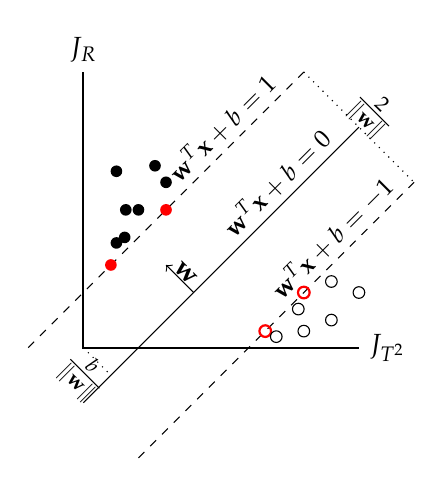
\begin{tikzpicture}[scale = 0.7]
  % Draw axes
  \draw [thick] (0,5) node (yaxis) [above] {$J_R$}
        |-(5,0) node (xaxis) [right] {$J_{T^2}$};
  % draw line
  \draw (0,-1) -- (5,4); % y=x-1
  \draw[dashed] (-1,0) -- (4,5); % y=x+1
  \draw[dashed] (1,-2) -- (6,3); % y=x-3
  % \draw labels
  \draw (3.5,3) node[rotate=45,font=\small] 
        {$\mathbf{w}^T \mathbf{x} + b = 0$};
  \draw (2.5,4) node[rotate=45,font=\small] 
        {$\mathbf{w}^T \mathbf{x} + b = 1$};
  \draw (4.5,2) node[rotate=45,font=\small] 
        {$\mathbf{w}^T \mathbf{x} + b = -1$};
  % draw distance
  \draw[dotted] (4,5) -- (6,3);
  \draw (5.25,4.25) node[rotate=-45] {$\frac{2}{\Vert \mathbf{w} \Vert}$};
  \draw[dotted] (0,0) -- (0.5,-0.5);
  \draw (0,-0.5) node[rotate=-45] {$\frac{b}{\Vert \mathbf{w} \Vert}$};
  \draw [->] (2,1) -- (1.5,1.5);
  \draw (1.85,1.35) node[rotate=-45] {$\mathbf{w}$};
  % draw negative dots
  \fill[red] (0.5,1.5) circle (3pt);
  \fill[red]   (1.5,2.5)   circle (3pt);
  \fill[black] (1,2.5)     circle (3pt);
  \fill[black] (0.75,2)    circle (3pt);
  \fill[black] (0.6,1.9)   circle (3pt);
  \fill[black] (0.77, 2.5) circle (3pt);
  \fill[black] (1.5,3)     circle (3pt);
  \fill[black] (1.3,3.3)   circle (3pt);
  \fill[black] (0.6,3.2)   circle (3pt);
 % \fill[black] (0.5,1)     circle (3pt);  % the outlier of the data
 % \fill[black] (2,0.5)     circle (3pt);
  % draw positive dots
  \draw[red,thick] (4,1)     circle (3pt); 
  \draw[red,thick] (3.3,.3)  circle (3pt); 
  \draw[black]     (4.5,1.2) circle (3pt); 
  \draw[black]     (4.5,.5)  circle (3pt); 
  \draw[black]     (3.9,.7)  circle (3pt); 
  \draw[black]     (5,1)     circle (3pt); 
  \draw[black]     (3.5,.2)  circle (3pt); 
  \draw[black]     (4,.3)    circle (3pt); 
 % \draw[black]     (3,1.5)   circle (3pt); % the outlier of the data
 % \draw[black]     (2,2)     circle (3pt);
\end{tikzpicture}
            \end{figure}
        \end{column}
    \end{columns}
\end{frame}

\begin{frame}{Support Vector Machine(soft margin)}
 \begin{columns}
 \begin{column}{0.5\textwidth}
  \begin{equation} \nonumber
     \begin{aligned}
     &\min\limits_{w,b,\xi}\frac{1}{2}{\parallel \omega  \parallel}^2 
     + C \sum\limits_{i=1}^{N}\xi_i
     \\
     &s.t. y_i(w^Tx_i+b)\geq 1 - \xi_i, & i = 1,2,\dots,N 
     \\
     &\xi_i \geq 0  & i= 1,2,\dots,N
     \end{aligned}
     \label{noSeparable}
 \end{equation}
        \end{column}
        \begin{column}{0.5\textwidth}  %%<--- here
            \begin{figure}[!htb] 
                \centering 
                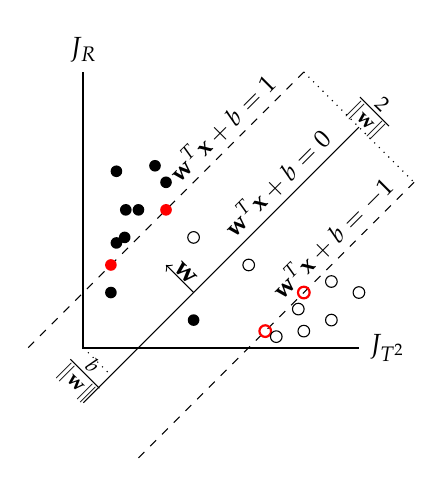
\begin{tikzpicture}[scale = 0.7]
  % Draw axes
  \draw [thick] (0,5) node (yaxis) [above] {$J_R$}
        |-(5,0) node (xaxis) [right] {$J_{T^2}$};
  % draw line
  \draw (0,-1) -- (5,4); % y=x-1
  \draw[dashed] (-1,0) -- (4,5); % y=x+1
  \draw[dashed] (1,-2) -- (6,3); % y=x-3
  % \draw labels
  \draw (3.5,3) node[rotate=45,font=\small] 
        {$\mathbf{w}^T \mathbf{x} + b = 0$};
  \draw (2.5,4) node[rotate=45,font=\small] 
        {$\mathbf{w}^T \mathbf{x} + b = 1$};
  \draw (4.5,2) node[rotate=45,font=\small] 
        {$\mathbf{w}^T \mathbf{x} + b = -1$};
  % draw distance
  \draw[dotted] (4,5) -- (6,3);
  \draw (5.25,4.25) node[rotate=-45] {$\frac{2}{\Vert \mathbf{w} \Vert}$};
  \draw[dotted] (0,0) -- (0.5,-0.5);
  \draw (0,-0.5) node[rotate=-45] {$\frac{b}{\Vert \mathbf{w} \Vert}$};
  \draw [->] (2,1) -- (1.5,1.5);
  \draw (1.85,1.35) node[rotate=-45] {$\mathbf{w}$};
  % draw negative dots
  \fill[red] (0.5,1.5) circle (3pt);
  \fill[red]   (1.5,2.5)   circle (3pt);
  \fill[black] (1,2.5)     circle (3pt);
  \fill[black] (0.75,2)    circle (3pt);
  \fill[black] (0.6,1.9)   circle (3pt);
  \fill[black] (0.77, 2.5) circle (3pt);
  \fill[black] (1.5,3)     circle (3pt);
  \fill[black] (1.3,3.3)   circle (3pt);
  \fill[black] (0.6,3.2)   circle (3pt);
  \fill[black] (0.5,1)     circle (3pt);  % the outlier of the data
  \fill[black] (2,0.5)     circle (3pt);
  % draw positive dots
  \draw[red,thick] (4,1)     circle (3pt); 
  \draw[red,thick] (3.3,.3)  circle (3pt); 
  \draw[black]     (4.5,1.2) circle (3pt); 
  \draw[black]     (4.5,.5)  circle (3pt); 
  \draw[black]     (3.9,.7)  circle (3pt); 
  \draw[black]     (5,1)     circle (3pt); 
  \draw[black]     (3.5,.2)  circle (3pt); 
  \draw[black]     (4,.3)    circle (3pt); 
  \draw[black]     (3,1.5)   circle (3pt); % the outlier of the data
  \draw[black]     (2,2)     circle (3pt);
\end{tikzpicture}
            \end{figure}
        \end{column}
    \end{columns}
\end{frame}



\section{The algorithm to find the threshold}


\begin{frame}{SMO algorithm}
The \href{https://www.microsoft.com/en-us/research/wp-content/uploads/2016/02/tr-98-14.pdf}{SMO}(Sequential Minimal Optimization) algorithm can find a set of $\alpha$.
Through the set of $ \alpha $, we can calculate the weights \textbf{w} and \textbf{b}.
\begin{equation}
    \begin{aligned}
   & \underset{\alpha}{\min}&&L(\alpha)=\frac{1}{2}\sum_{i=1}^{N}\sum_{j=1}^{N}
    \alpha_i\alpha_jy_iy_jK(x_i,x_j)-\sum_{i=1}^{N}\alpha_i \\
   & \text{subject to} &&\sum_{i=1}^{N}\alpha_iy_i=0 \\
   & && 0 \leq\alpha_i\leq C 
    \end{aligned}
    \label{Cons_cond}
\end{equation}
\begin{equation}
 w =\sum_{i=1}^N\alpha_i y_ix_i
 \end{equation}
\end{frame}

\begin{frame}{SMO algorithm}
 \begin{columns}
             \begin{column}{0.5\textwidth}
object: w,b \par
Steps:
\begin{enumerate}
    \item Initialize the value of multiplier $\alpha$
    \item Find a multiplier $\alpha_1^{old}$ 
    \item Pick another multiplier $\alpha_2^{old}$
    \item Compute the $\alpha_1^{new},\alpha_2^{new}$
    \item Updata the value of b
    \item Repeat the above steps until convergence
\end{enumerate}

           \end{column}
        \begin{column}{0.5\textwidth}  %%<--- here
    \begin{equation} \nonumber
    \begin{aligned}
    &g(x) = \sum_{i=1}^{N}\alpha_iy_iK(x_i,x)+b \\
 &E_i = g(x_i)-y_i \quad i = 1,2 \\
&\eta = K_{11}+K_{22}-2K_{12} \\
&\alpha_2^{new,unc}= \alpha_2^{old}+\frac{y_2(E_1-E_2)}{\eta}
    \end{aligned}
\end{equation}
 \begin{equation} \nonumber
    \alpha_2^{new}=\left\{
\begin{aligned}
&H,  &&\alpha_2^{new,unc}>H\\
&\alpha_2^{new,unc}, &&L\leq \alpha_2^{new,unc}\leq H\\
&L, &&\alpha_2^{new,unc}<L
\end{aligned}
\right.
\end{equation}
\begin{equation} \nonumber
\alpha_1^{new} =    \alpha_1^{old}+y_1y_2(\alpha_2^{old}-\alpha_2^{new})
\end{equation}
        \end{column}
    \end{columns}
\end{frame}
\begin{frame}{Tune hyperplane based on FAR or FDR}
 \begin{columns}
             \begin{column}{0.5\textwidth}
               SMO algorithm  $\rightarrow$ (w,b) \par
The hyperplane: \par
            $
             w^Tx+b = 0
            $  \par
 The decision function: \par
$
  \begin{aligned}
  & f(x) =  
 w^Tx_i+b  \\
  & D = \left\{
     \begin{aligned}
      &-1\quad &f(x)<0   \\
      &\quad 1    \quad &f(x)>0 
     \end{aligned}
  \right. 
    \end{aligned}
$
            
           \end{column}
        \begin{column}{0.5\textwidth}  %%<--- here
            \begin{figure}[!htb] 
                \centering 
                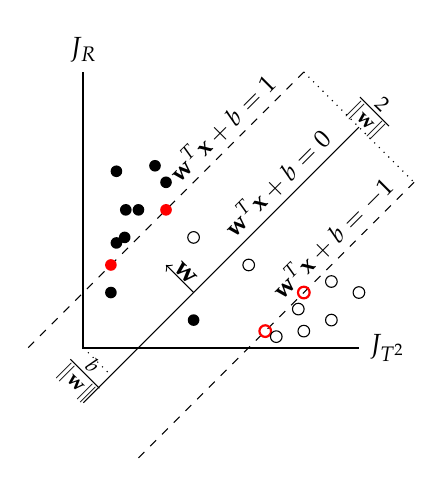
\begin{tikzpicture}[scale = 0.7]
  % Draw axes
  \draw [thick] (0,5) node (yaxis) [above] {$J_R$}
        |-(5,0) node (xaxis) [right] {$J_{T^2}$};
  % draw line
  \draw (0,-1) -- (5,4); % y=x-1
  \draw[dashed] (-1,0) -- (4,5); % y=x+1
  \draw[dashed] (1,-2) -- (6,3); % y=x-3
  % \draw labels
  \draw (3.5,3) node[rotate=45,font=\small] 
        {$\mathbf{w}^T \mathbf{x} + b = 0$};
  \draw (2.5,4) node[rotate=45,font=\small] 
        {$\mathbf{w}^T \mathbf{x} + b = 1$};
  \draw (4.5,2) node[rotate=45,font=\small] 
        {$\mathbf{w}^T \mathbf{x} + b = -1$};
  % draw distance
  \draw[dotted] (4,5) -- (6,3);
  \draw (5.25,4.25) node[rotate=-45] {$\frac{2}{\Vert \mathbf{w} \Vert}$};
  \draw[dotted] (0,0) -- (0.5,-0.5);
  \draw (0,-0.5) node[rotate=-45] {$\frac{b}{\Vert \mathbf{w} \Vert}$};
  \draw [->] (2,1) -- (1.5,1.5);
  \draw (1.85,1.35) node[rotate=-45] {$\mathbf{w}$};
  % draw negative dots
  \fill[red] (0.5,1.5) circle (3pt);
  \fill[red]   (1.5,2.5)   circle (3pt);
  \fill[black] (1,2.5)     circle (3pt);
  \fill[black] (0.75,2)    circle (3pt);
  \fill[black] (0.6,1.9)   circle (3pt);
  \fill[black] (0.77, 2.5) circle (3pt);
  \fill[black] (1.5,3)     circle (3pt);
  \fill[black] (1.3,3.3)   circle (3pt);
  \fill[black] (0.6,3.2)   circle (3pt);
  \fill[black] (0.5,1)     circle (3pt);  % the outlier of the data
  \fill[black] (2,0.5)     circle (3pt);
  % draw positive dots
  \draw[red,thick] (4,1)     circle (3pt); 
  \draw[red,thick] (3.3,.3)  circle (3pt); 
  \draw[black]     (4.5,1.2) circle (3pt); 
  \draw[black]     (4.5,.5)  circle (3pt); 
  \draw[black]     (3.9,.7)  circle (3pt); 
  \draw[black]     (5,1)     circle (3pt); 
  \draw[black]     (3.5,.2)  circle (3pt); 
  \draw[black]     (4,.3)    circle (3pt); 
  \draw[black]     (3,1.5)   circle (3pt); % the outlier of the data
  \draw[black]     (2,2)     circle (3pt);
\end{tikzpicture}
            \end{figure}
        \end{column}
    \end{columns}
\end{frame}
\begin{frame}{Tune hyperplane based on FAR or FDR}
Assume $D = -1$ is fault-free, $FAR = \alpha$,$FDR =\beta$, large enough sample condition is satisfied.\par
The (practical) FD specific requirements: \par
$Pr(D=1|f=0)\leq \alpha$ or\par
$Pr(D=1|f \neq 0)\geq \beta$ \par
If the requirements are not meet: \par
$Pr(D=1|f=0)> \alpha$ or\par
$Pr(D=1|f \neq 0) < \beta$ \par
how to solve the problem?
\end{frame}

\begin{frame}{Tune hyperplane based on FAR or FDR}
\href{https://ieeexplore.ieee.org/abstract/document/8306878}{FAR}: $Pr(D=1|f=0) \approx \frac{1}{n_1}\sum_{i=1}^{n_1}I_{i-}$  \par
\href{https://ieeexplore.ieee.org/abstract/document/8306878}{FDR}: $Pr(D=1|f \neq 0) \approx          \frac{1}{n_2}\sum_{j=1}^{n_2}I_{j+}$ \par
\begin{equation}
I_{i-} = \left\{ \begin{aligned}
0 \quad  w^Tx_{n_i} + b < 0 \\
1 \quad w^Tx_{n_i} +b  > 0 
\end{aligned}
\right.
\end{equation}
where $x_n$ is fault-free data, $i=1,2,\dots,n_1$
\begin{equation}
I_{i+} = \left\{ \begin{aligned}
0 \quad  w^Tx_{f_j} + b < 0 \\
1 \quad w^Tx_{f_j} +b  > 0 
\end{aligned}
\right.
\end{equation}
where $x_f$ is faulty data, $j=1,2,\dots,n_2$
\end{frame}
\begin{frame}{Tune hyperplane based on FAR}
 \begin{columns}
             \begin{column}{0.5\textwidth}
    Idea: change b to meet FAR or FDR requirements. \par
Case 1: $Pr(D=1|f=0) > \alpha$
\begin{exampleblock}{Steps}
      \begin{enumerate}
      \item Giving a small step length $\epsilon > 0$
      \item $b = b - \epsilon$, updating the decision function
      \item Computing  $Pr(D=1|f=0)$
      \item If  $Pr(D=1|f=0) > \alpha$, then go to the step 2 
 	 \end{enumerate}  
 	 \end{exampleblock}
           \end{column}
        \begin{column}{0.5\textwidth}  %%<--- here
    \begin{figure}[!htb] 
                \centering 
                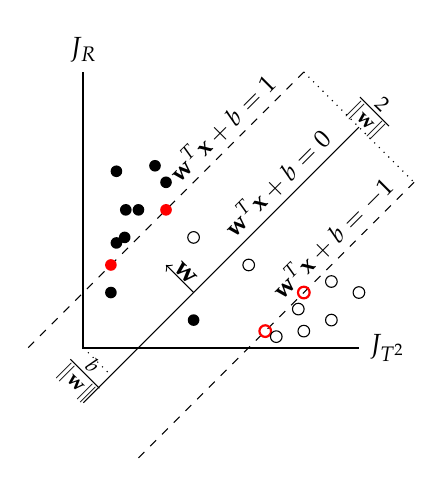
\begin{tikzpicture}[scale = 0.7]
  % Draw axes
  \draw [thick] (0,5) node (yaxis) [above] {$J_R$}
        |-(5,0) node (xaxis) [right] {$J_{T^2}$};
  % draw line
  \draw (0,-1) -- (5,4); % y=x-1
  \draw[dashed] (-1,0) -- (4,5); % y=x+1
  \draw[dashed] (1,-2) -- (6,3); % y=x-3
  % \draw labels
  \draw (3.5,3) node[rotate=45,font=\small] 
        {$\mathbf{w}^T \mathbf{x} + b = 0$};
  \draw (2.5,4) node[rotate=45,font=\small] 
        {$\mathbf{w}^T \mathbf{x} + b = 1$};
  \draw (4.5,2) node[rotate=45,font=\small] 
        {$\mathbf{w}^T \mathbf{x} + b = -1$};
  % draw distance
  \draw[dotted] (4,5) -- (6,3);
  \draw (5.25,4.25) node[rotate=-45] {$\frac{2}{\Vert \mathbf{w} \Vert}$};
  \draw[dotted] (0,0) -- (0.5,-0.5);
  \draw (0,-0.5) node[rotate=-45] {$\frac{b}{\Vert \mathbf{w} \Vert}$};
  \draw [->] (2,1) -- (1.5,1.5);
  \draw (1.85,1.35) node[rotate=-45] {$\mathbf{w}$};
  % draw negative dots
  \fill[red] (0.5,1.5) circle (3pt);
  \fill[red]   (1.5,2.5)   circle (3pt);
  \fill[black] (1,2.5)     circle (3pt);
  \fill[black] (0.75,2)    circle (3pt);
  \fill[black] (0.6,1.9)   circle (3pt);
  \fill[black] (0.77, 2.5) circle (3pt);
  \fill[black] (1.5,3)     circle (3pt);
  \fill[black] (1.3,3.3)   circle (3pt);
  \fill[black] (0.6,3.2)   circle (3pt);
  \fill[black] (0.5,1)     circle (3pt);  % the outlier of the data
  \fill[black] (2,0.5)     circle (3pt);
  % draw positive dots
  \draw[red,thick] (4,1)     circle (3pt); 
  \draw[red,thick] (3.3,.3)  circle (3pt); 
  \draw[black]     (4.5,1.2) circle (3pt); 
  \draw[black]     (4.5,.5)  circle (3pt); 
  \draw[black]     (3.9,.7)  circle (3pt); 
  \draw[black]     (5,1)     circle (3pt); 
  \draw[black]     (3.5,.2)  circle (3pt); 
  \draw[black]     (4,.3)    circle (3pt); 
  \draw[black]     (3,1.5)   circle (3pt); % the outlier of the data
  \draw[black]     (2,2)     circle (3pt);
\end{tikzpicture}
            \end{figure}
  
        \end{column}
    \end{columns}
\end{frame}

\begin{frame}{Tune hyperplane based on FDR}
 \begin{columns}
             \begin{column}{0.5\textwidth}
    
    Case 2: $Pr(D=1|f\neq 0) < \beta$
\begin{exampleblock}{Steps}
      \begin{enumerate}
      \item Giving a small step length $\epsilon > 0$
      \item $b = b + \epsilon$, updating the decision function
      \item Computing  $Pr(D=1|f\neq 0)$
      \item If  $Pr(D=1|f\neq 0) < \beta$, then go to the step 2 
 	 \end{enumerate}  
 	 \end{exampleblock}
           \end{column}
        \begin{column}{0.5\textwidth}  %%<--- here
    \begin{figure}[!htb] 
                \centering 
                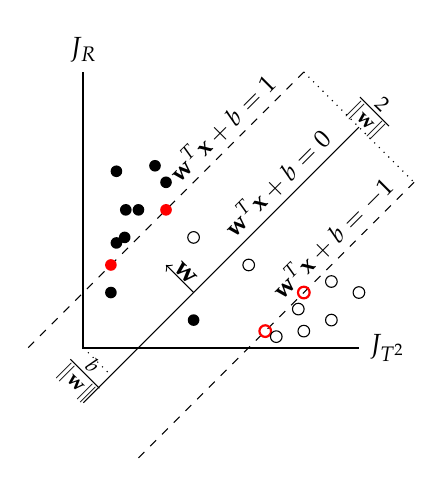
\begin{tikzpicture}[scale = 0.7]
  % Draw axes
  \draw [thick] (0,5) node (yaxis) [above] {$J_R$}
        |-(5,0) node (xaxis) [right] {$J_{T^2}$};
  % draw line
  \draw (0,-1) -- (5,4); % y=x-1
  \draw[dashed] (-1,0) -- (4,5); % y=x+1
  \draw[dashed] (1,-2) -- (6,3); % y=x-3
  % \draw labels
  \draw (3.5,3) node[rotate=45,font=\small] 
        {$\mathbf{w}^T \mathbf{x} + b = 0$};
  \draw (2.5,4) node[rotate=45,font=\small] 
        {$\mathbf{w}^T \mathbf{x} + b = 1$};
  \draw (4.5,2) node[rotate=45,font=\small] 
        {$\mathbf{w}^T \mathbf{x} + b = -1$};
  % draw distance
  \draw[dotted] (4,5) -- (6,3);
  \draw (5.25,4.25) node[rotate=-45] {$\frac{2}{\Vert \mathbf{w} \Vert}$};
  \draw[dotted] (0,0) -- (0.5,-0.5);
  \draw (0,-0.5) node[rotate=-45] {$\frac{b}{\Vert \mathbf{w} \Vert}$};
  \draw [->] (2,1) -- (1.5,1.5);
  \draw (1.85,1.35) node[rotate=-45] {$\mathbf{w}$};
  % draw negative dots
  \fill[red] (0.5,1.5) circle (3pt);
  \fill[red]   (1.5,2.5)   circle (3pt);
  \fill[black] (1,2.5)     circle (3pt);
  \fill[black] (0.75,2)    circle (3pt);
  \fill[black] (0.6,1.9)   circle (3pt);
  \fill[black] (0.77, 2.5) circle (3pt);
  \fill[black] (1.5,3)     circle (3pt);
  \fill[black] (1.3,3.3)   circle (3pt);
  \fill[black] (0.6,3.2)   circle (3pt);
  \fill[black] (0.5,1)     circle (3pt);  % the outlier of the data
  \fill[black] (2,0.5)     circle (3pt);
  % draw positive dots
  \draw[red,thick] (4,1)     circle (3pt); 
  \draw[red,thick] (3.3,.3)  circle (3pt); 
  \draw[black]     (4.5,1.2) circle (3pt); 
  \draw[black]     (4.5,.5)  circle (3pt); 
  \draw[black]     (3.9,.7)  circle (3pt); 
  \draw[black]     (5,1)     circle (3pt); 
  \draw[black]     (3.5,.2)  circle (3pt); 
  \draw[black]     (4,.3)    circle (3pt); 
  \draw[black]     (3,1.5)   circle (3pt); % the outlier of the data
  \draw[black]     (2,2)     circle (3pt);
\end{tikzpicture}
            \end{figure}
  
        \end{column}
    \end{columns}

\end{frame}
\section{Case study}
\begin{frame}{Generating the data}
    $y = y_n + f, \left\{ \begin{aligned}
    f = 0      \quad &\text{fault-free} \\
    f \neq 0   \quad &\text{additive faults}
     \end{aligned} 
     \right. $
   $y = My_n,\left\{ \begin{aligned}
    M = Id     \quad &\text{fault-free} \\
    M \neq Id   \quad &\text{multiplicative faults}
     \end{aligned} 
     \right. $
     \metroset{block=fill}
      \begin{exampleblock}{Relation}
	\begin{itemize}
    \item \href{https://ieeexplore.ieee.org/document/8425029}{Changes in mean can be mapped to additive faults} 
    \item \href{https://ieeexplore.ieee.org/document/8425029}{Changes in variance can be mapped to multiplicative faults}
    \end{itemize}
    \end{exampleblock}
    
\end{frame}
\begin{frame}{Generating the data}
 \begin{columns}
             \begin{column}{0.5\textwidth}
    \begin{center}
\begin{tabular}{ccc}
\hline
y& number& Distribution                                    \\
\hline
$y_n  $ &$n_1$& $y_n \sim N(\mu, \sigma^2)$                \\
$y_a  $ &$n_2$& $y_{a_i} \sim N(\mu_i,\sigma^2$)           \\
$y_m  $ &$n_3$& $y_{m_j} \sim N(\mu,\sigma_j^2)$           \\
%  $y_{am}$&$n_4$& $y_{am_k}\sim N(\mu_k,\sigma_k^2)$         \\
$y_{ms}$ &$n_4$& $y_{ms_k} \sim N(\mu,\sigma_k^2)$  \\
\hline
\end{tabular}
\end{center}
where $\mu \neq \mu_i,\sigma < \sigma_j,\sigma > \sigma_k$. \par Every \textbf{p} samples as a group
$y_{a_i},y_{m_j},y_{ms_k}$. \par $i = 1,2,\dots,\frac{n_2}{p},j=1,2,\dots,\frac{n_3}{p}$ \par
$k = 1,2,\dots,\frac{n_4}{p}$
           \end{column}
        \begin{column}{0.5\textwidth}  %%<--- here
   \begin{figure}
        \centering
        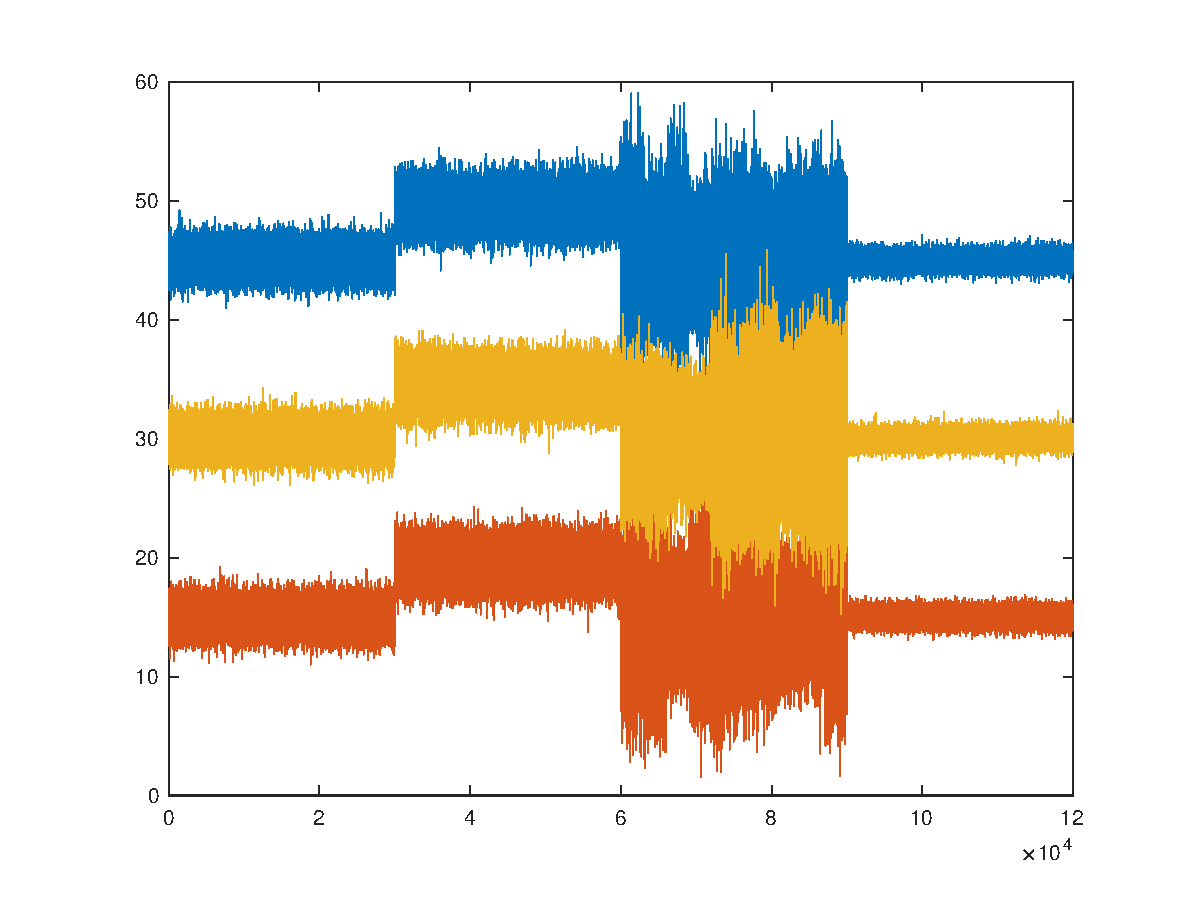
\includegraphics[width=6cm]{fig/four.eps} %Coriginal.eps
    \end{figure}
    $\hspace{1.2cm} y_n \hspace{1cm} y_a \hspace{0.7cm} y_m  \hspace{0.7cm} y_{ms}$
        \end{column}
    \end{columns}
\end{frame}
\begin{frame}{Case study on a numerical example}
     \begin{columns}
             \begin{column}{0.6\textwidth}
              \begin{figure}
              \centering
           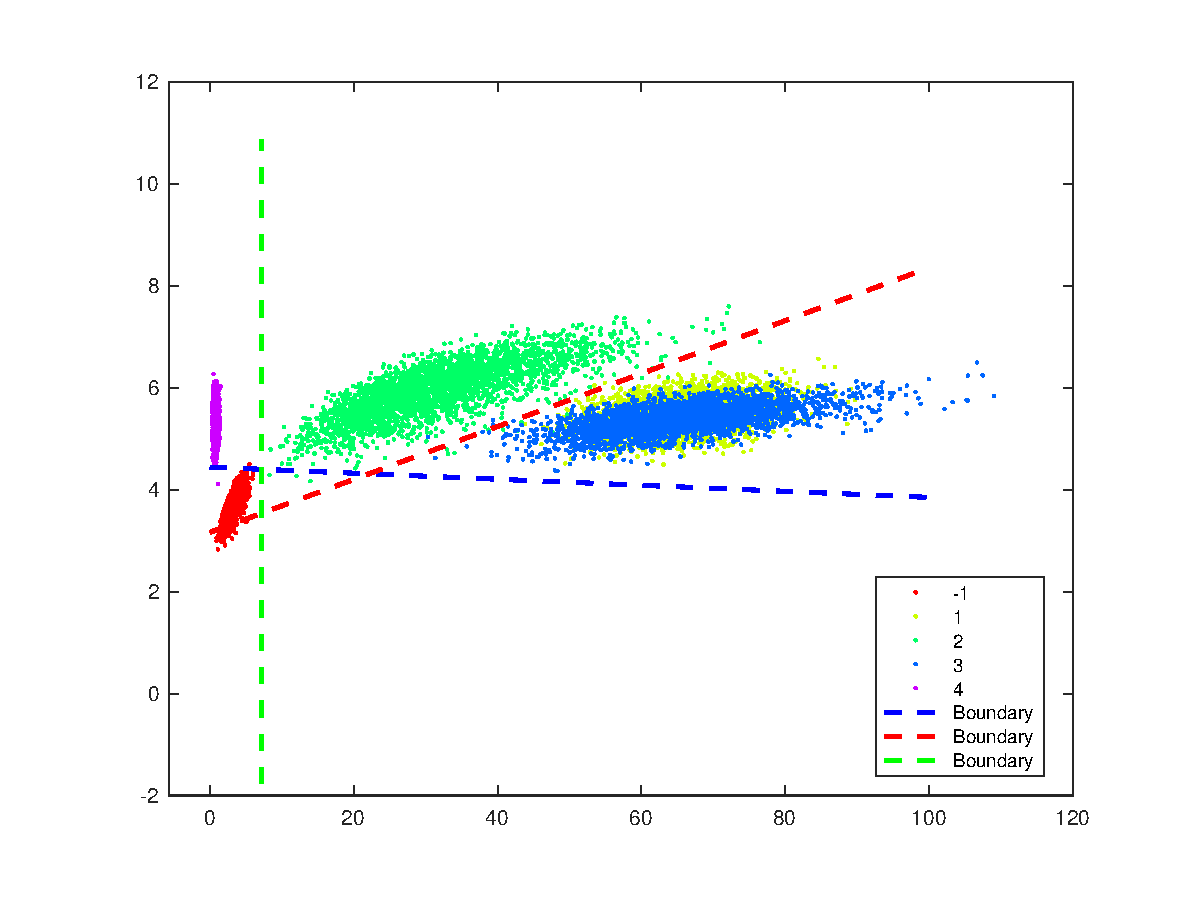
\includegraphics[width=5cm]{fig/perfectR.eps}
            \end{figure}
            \begin{equation} \nonumber
            \begin{aligned}
         &w_r^T = [0.2859  \quad  -0.1169] \quad &b_r =  -1.7315 \\
         &w_g^T = [0.8847 \quad 0.0007]\quad &b_g =-6.3180  \\
         &w_b^T = [0.0481 \quad 5.2780] \quad &b_b = -23.5837  \\
           \end{aligned}
            \end{equation}
           \end{column}
        \begin{column}{0.4\textwidth}  %%<--- here
        \textcolor{red}{Decision rule:}    \par
         $f_r(x)=w_r^Tx+b_r $ \par
         $f_g(x)=w_g^Tx+b_g $ \par
         $f_b(x) = w_b^Tx+b_b$ \par 
         \begin{enumerate}
             \item $f_b(x_i)<0,f_g(x_i)< 0$ 
             \item $f_b(x_i)>0,f_g(x_i)< 0$
             \item $f_b(x_i),f_g(x_i),f_r(x_i)>0$
             \item $f_b(x_i)>0,f_r(x_i)<0$
         \end{enumerate}
        \end{column}
    \end{columns}
\end{frame}
\begin{frame}{Case study on three-tank system(TTS)}
\begin{columns}
         \begin{column}{0.5\textwidth}
         \begin{equation}
         \begin{aligned}
     &\dot{x}=(A+\Delta A_F)x + Bu + E_ff  \\
     &y = Cx+F_ff
     \end{aligned}
 \end{equation}    
        $w^T = [0.0481 \quad 5.2780]$ $b = -23.5837$
    \begin{equation} \nonumber
  \begin{aligned}
   & FAR \approx \frac{14}{14+882331} \approx 1.5867\times 10^{-3} \% \\
   & FDR \approx 1 - \frac{48651}{48651+933651} \approx 95.05 \% \\
   & VA \approx 1 - \frac{48651+14}{933651+882331} \approx 97.32 \%
  \end{aligned}
\end{equation}
   \par
   VA: validation accuracy
           \end{column}
        \begin{column}{0.5\textwidth}  %%<--- here
   \begin{figure}
        \centering
        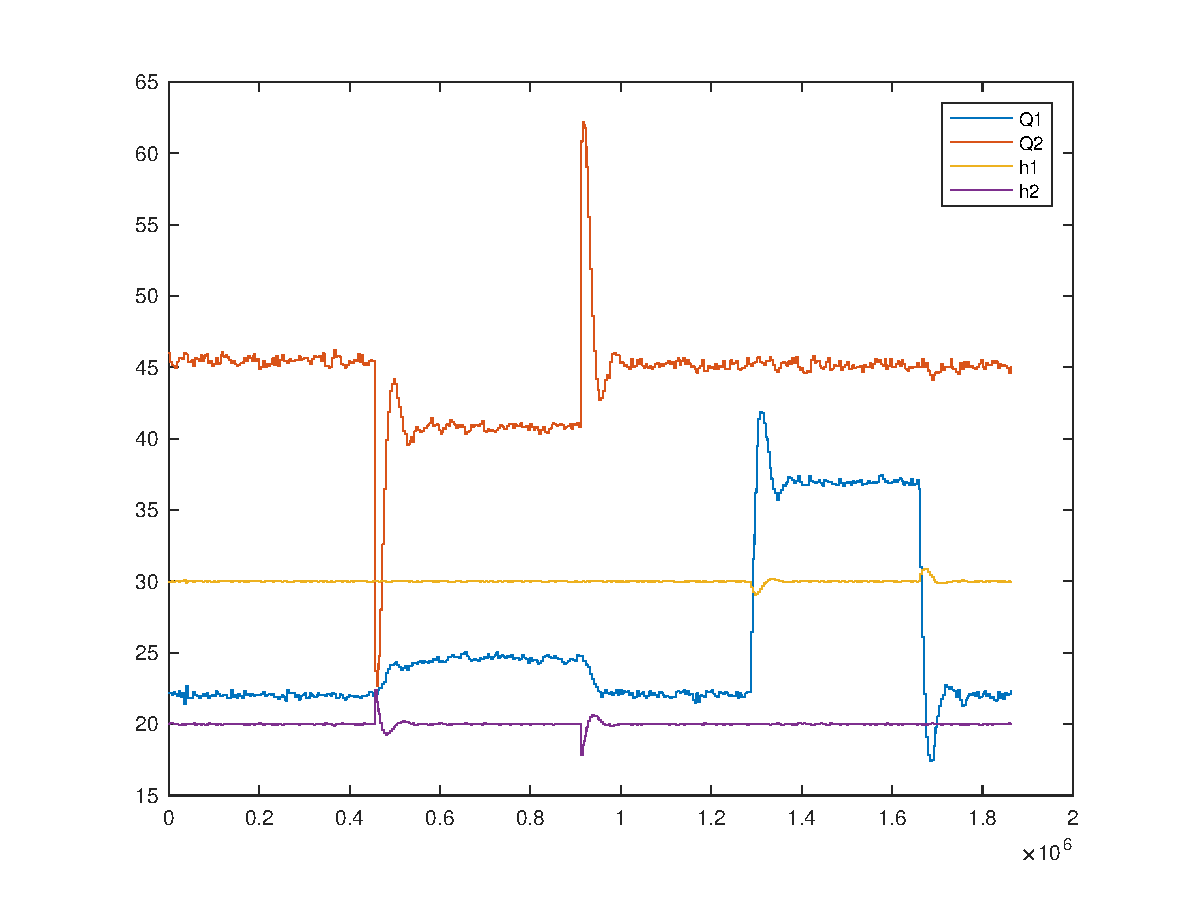
\includegraphics[width=4cm]{fig/realori.eps}
        \caption{real data from TTS}
        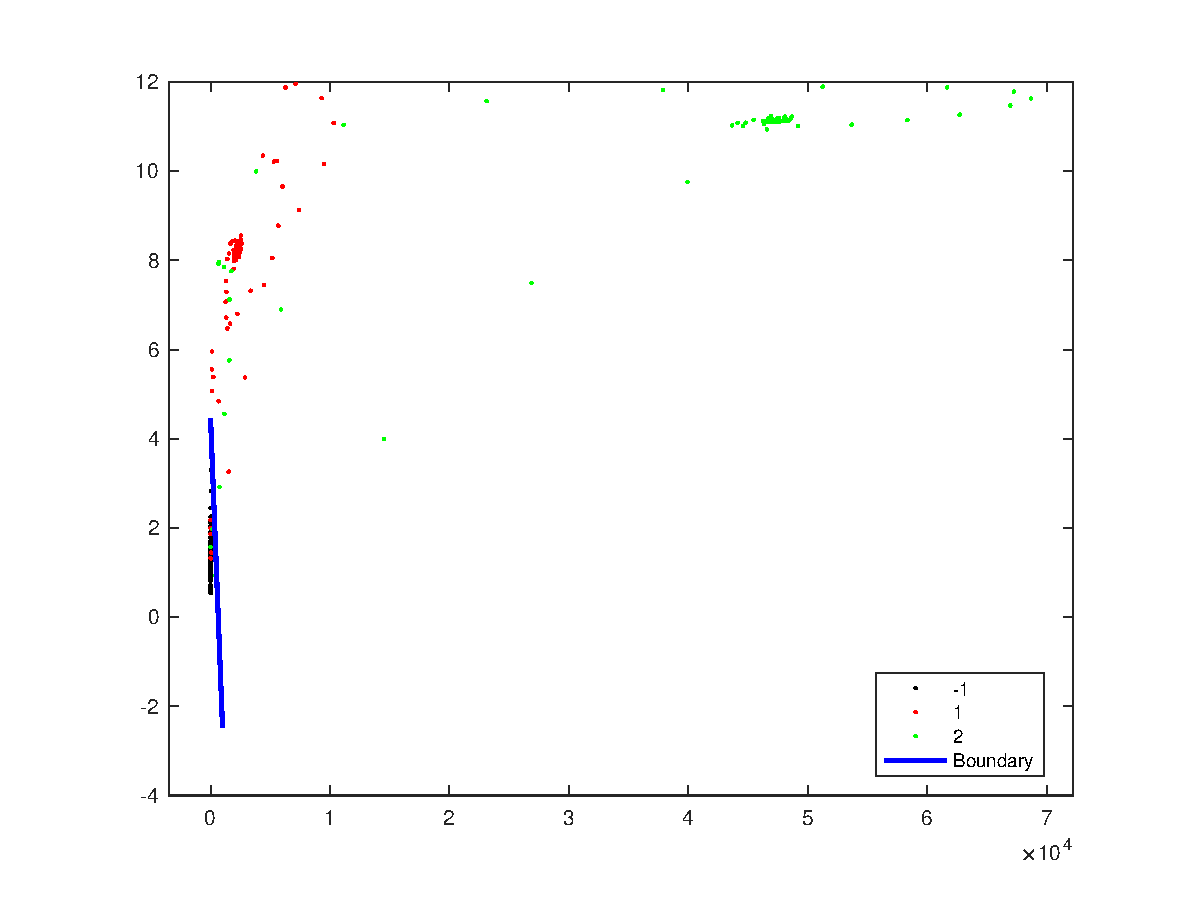
\includegraphics[width=4cm]{fig/realdata.eps}
        \caption{The hyperplane of the data}
        \end{figure}
  
        \end{column}
    \end{columns}
\end{frame}

\begin{frame}{Case study on continuous stirred tank heater(CSTH)}
     \begin{columns}
             \begin{column}{0.5\textwidth}
 $w^T = [0.1775 \quad 2.2058]$,$b = -7.1464$
 \begin{equation} \nonumber
  \begin{aligned}
  & f(x) =  
 w^Tx_i+b  \\
  & D = \left\{
     \begin{aligned}
      &-1\quad &f(x)<0 \quad &\text{(fault-free)}  \\
      &\quad 1    \quad &f(x)>0 \quad &\text{(faulty)}
     \end{aligned}
  \right. 
    \end{aligned}
\end{equation}
\begin{equation} \nonumber
  \begin{aligned}
   & FAR \approx \frac{1}{1+1142} \approx  8.7489\times 10^{-2} \% \\
   & FDR \approx 1 - \frac{0}{0+2743} \approx 100 \% \\
   & VA \approx 1 - \frac{1+0}{1143+2743} \approx 99.97 \% 
  \end{aligned}
\end{equation}
   \par
  VA: validation accuracy
           \end{column}
        \begin{column}{0.5\textwidth}  %%<--- here
   \begin{figure}
        \centering
        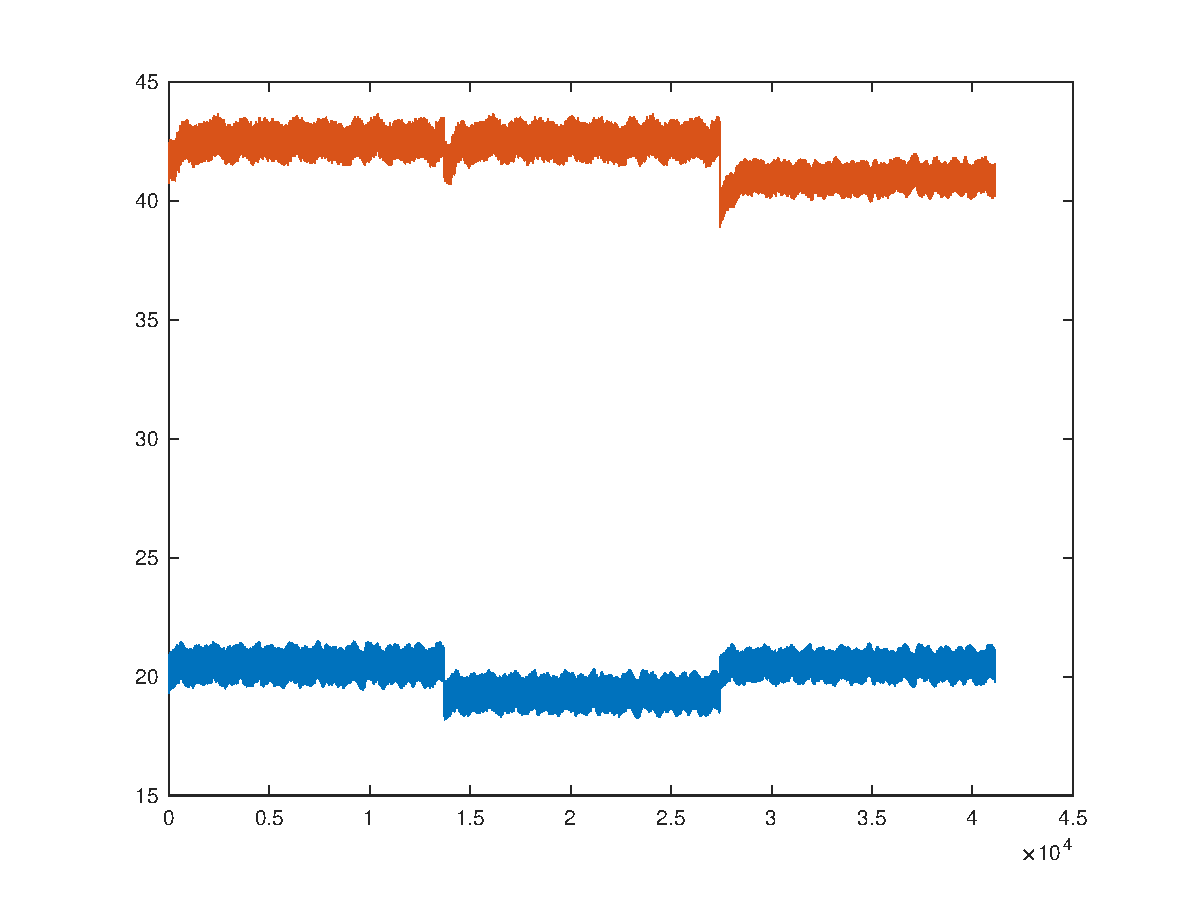
\includegraphics[width=4cm]{fig/csthrealdata.eps}
        \caption{data of CSTH}
        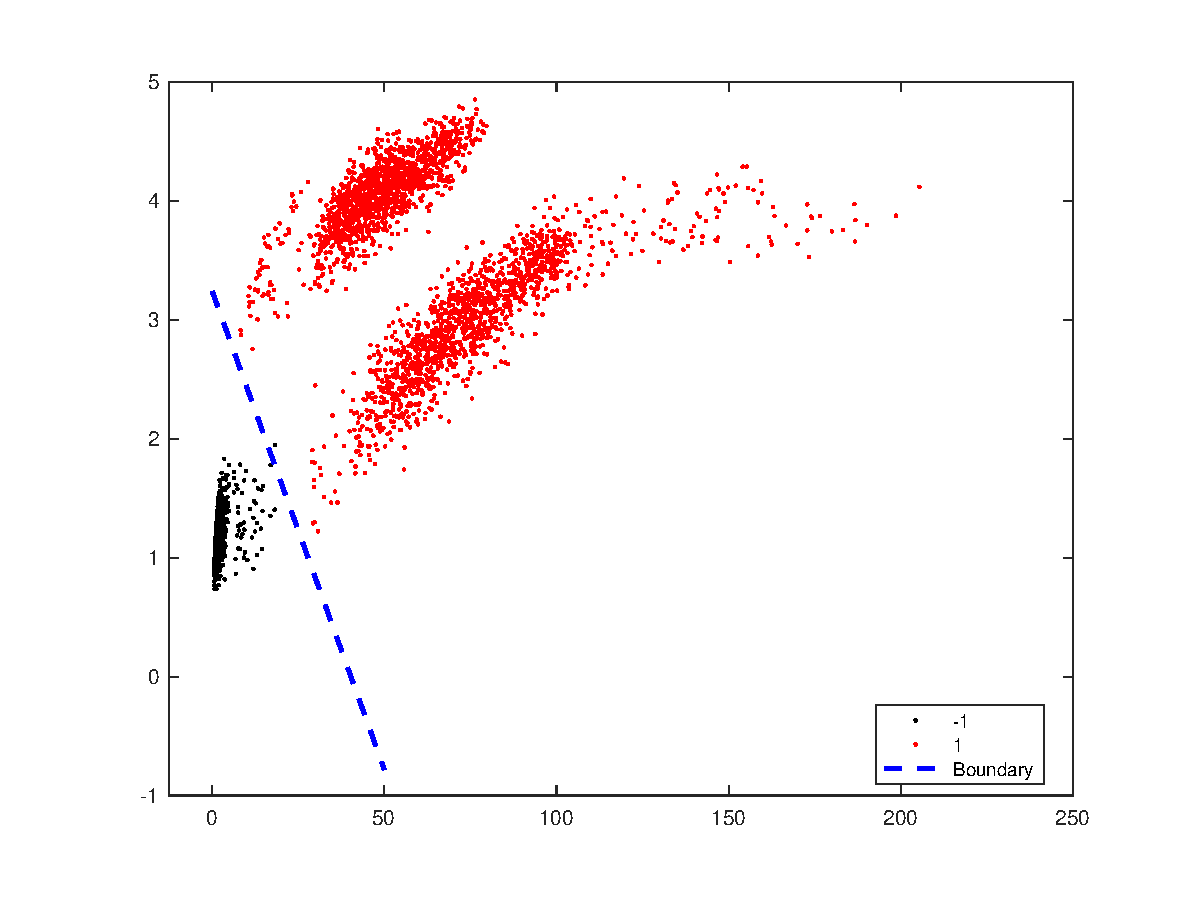
\includegraphics[width=4cm]{fig/Csthboundary.eps}
        \caption{The hyperplane of the data}
        \end{figure}
   
        \end{column}
    \end{columns}
\end{frame}
\section{Conclusion and future work}

\begin{frame}{Conclusion and future work}
Conclusion:
\begin{itemize}
    \item extract feature data using the $T^2$-statistic and Riemannian manifold
    \item find hyperplane
    \item tune hyperplane
    \item multi-hyperplanes separate the different types of data
\end{itemize}
Future work:
     \begin{itemize}
      \item \textcolor{blue}{1}: Combine 3 FD methods using SVM
      \item \textcolor{blue}{3}: Randomized algorithms to find the threshold of two-dimensional data 
 	 \end{itemize}  
\end{frame}

\begin{frame}[standout]
\begin{center}
Thank you for your attention!
\end{center}
\end{frame}

\section{Appendix}
\begin{frame}{Geometry of SPD Matrices}
An n $\times$ n square matrix M is SPD, if and only if
\begin{itemize}
    \item $M^T = M$
    \item $u^TMu>0$ and $\forall u \neq 0$
\end{itemize}
SPD matrices have the following properties:
\begin{itemize}
\item 1. $\forall$ M $\in$ SPD(n), $M^{-1}$ $\in$ SPD(n) i.e., SPD matrices are invertible. 
\item 2. $\forall$ M $\in$ SPD(n), eigenvalues are positive i.e., λ(M) > 0.
\end{itemize}
\end{frame}
\begin{frame}{Riemannian metric}
    \begin{columns}
        \begin{column}{0.5\textwidth}
          \begin{equation} \nonumber
          \begin{aligned}
          &S_i = C^{\frac{1}{2}}logm(C^{-\frac{1}{2}}C_iC^{-\frac{1}{2}})C^{\frac{1}{2}} \\
          &C_i = C^{\frac{1}{2}}expm(C^{-\frac{1}{2}}S_iC^{-\frac{1}{2}})C^{\frac{1}{2}} \\
          \end{aligned}
           \end{equation}
        \end{column}
        \begin{column}{0.5\textwidth}  %%<--- here
            \begin{figure}[!htb] 
                \centering 
               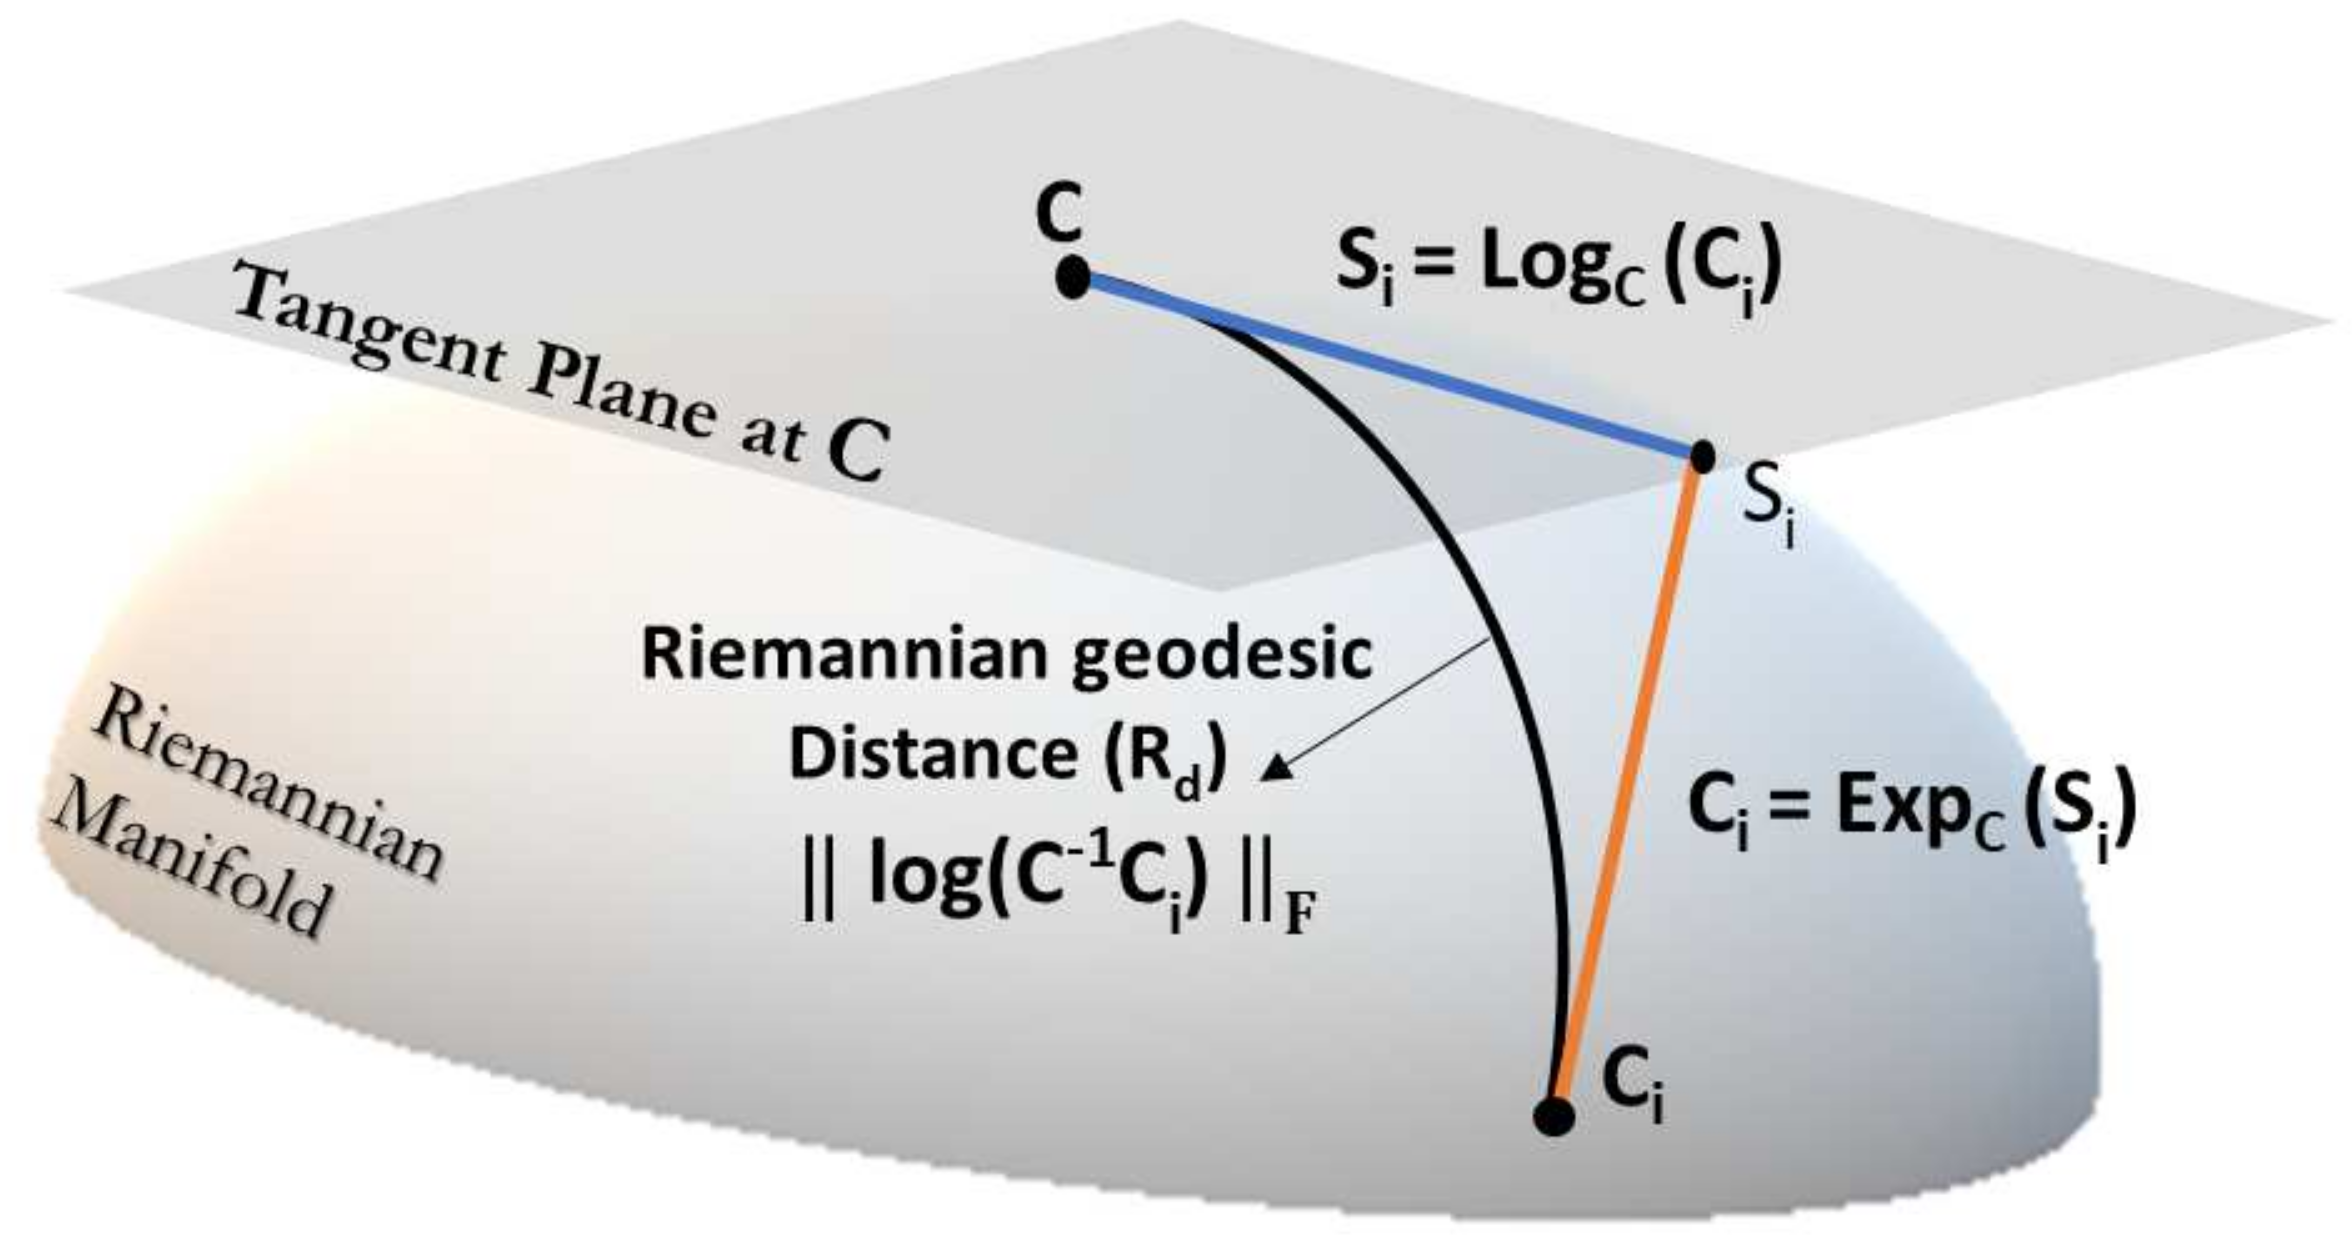
\includegraphics[width=0.7\textwidth]{RieDis.png}
               \caption{\href{https://www.mdpi.com/1424-8220/19/2/379}{Riemannian mainfold}} 
            \end{figure}
        \end{column}
    \end{columns}
\end{frame}
\begin{frame}{Support Vector Machine(linearly separable)}
\begin{equation}
L(w,b,\alpha) = \frac{1}{2}w^Tw-\sum_{i=1}^N\alpha_i(y_i(w^Tx+b)-1)
\end{equation}
\begin{equation}
    \begin{aligned}
&\frac{\partial{L}}{\partial{w}} = w - \sum_{i=1}^N\alpha y_ix_i = 0  \\
&\frac{\partial{L}}{\partial{b}} =- \sum_{i=1}^{N} \alpha_iy_i =0 
    \end{aligned} \label{Dif_wb}
\end{equation}
\begin{equation}
    \begin{aligned}
    w =\sum_{i=1}^N\alpha_i y_ix_i  \\
    \sum_{i=1}^{N} \alpha_iy_i = 0  \\ 
    \end{aligned}
    \label{wbValue}
\end{equation}
\begin{equation}
\underset{\alpha}{\max}L(\alpha)
=  \sum_{i=1}^N\alpha_i-\frac{1}{2}\sum_{i,j=1}^Ny_iy_j\alpha_i\alpha_j<x_i \cdot x_j>
    \label{o_wb}
\end{equation}
\end{frame}
\begin{frame}{SMO algorithm}
    When $y_1 \neq y_2$:
\begin{equation}
    \begin{aligned}
        & L = \max(0,\alpha_2^{old}-\alpha_1^{old}) \\
        & H = \min(C,C+\alpha_2^{old}-\alpha_1^{old})
    \end{aligned}
\end{equation}
when $y_1 = y_2$:
\begin{equation}
    \begin{aligned}
&    L = \max(0,\alpha_2^{old}+\alpha_1^{old}-C) \\
&    H = \min(C,\alpha_2^{old}+\alpha_1^{old})
    \end{aligned}
\end{equation}
\end{frame}

\begin{frame}{SMO algorithm}
Assume two variables $\alpha_1,\alpha_2$ are determined, rewrite the equation \ref{Cons_cond}:
\begin{equation}
    \underset{\alpha_1,\alpha_2}{\min}  L(\alpha)= \underset{\alpha_1,\alpha_2}{\min}W(\alpha_1,\alpha_2)
    +\frac{1}{2}\sum_{i=3}^{N}\sum_{j=3}^{N}\alpha_i\alpha_jy_iy_jK(x_i,x_j)-\sum_{i=3}^{N}\alpha_i
\end{equation}
\begin{equation}
    \begin{aligned}
    \underset{\alpha_1,\alpha_2}{\min}W(\alpha_1,\alpha_2)
   &=&&\frac{1}{2}K_{11}\alpha_1^2+\frac{1}{2}K_{22}\alpha_2^2-(\alpha_1+\alpha_2) \\
   & &&+y_1\alpha_1\sum_{i=3}^{N}y_i\alpha_iK_{i1}+y_2\alpha_2\sum_{i=3}^Ny_i\alpha_iK_{i2} \\
   &s.t.&&\alpha_1y_1+\alpha_2y_2 = -\sum_{i=3}^Ny_i\alpha_i = \zeta
    \end{aligned}
    \label{SMO_cond}
\end{equation}
where $\zeta$ is constant.
\end{frame}

\begin{frame}{SMO algorithm}
    \begin{equation}
    \begin{aligned}
    &g(x) = \sum_{i=1}^{N}\alpha_iy_iK(x_i,x)+b \\
 &E_i = g(x_i)-y_i= \left(\sum_{j=1}^N\alpha_jy_jK(x_j,x_i)+b\right)-y_i \quad i = 1,2 \\
&\eta = K_{11}+K_{22}-2K_{12} \\
&\alpha_2^{new,unc}= \alpha_2^{old}+\frac{y_2(E_1-E_2)}{\eta}
    \end{aligned}
\end{equation}
 \begin{equation}
    \alpha_2^{new}=\left\{
\begin{aligned}
&H,  &&\alpha_2^{new,unc}>H\\
&\alpha_2^{new,unc}, &&L\leq \alpha_2^{new,unc}\leq H\\
&L, &&\alpha_2^{new,unc}<L
\end{aligned}
\right.
\end{equation}
\begin{equation}
\alpha_1^{new} =    \alpha_1^{old}+y_1y_2(\alpha_2^{old}-\alpha_2^{new})
\end{equation}
\begin{equation}
b_1^{new}=-E_1-y_1K_{11}(\alpha_1^{new}-\alpha_1^{old})-y_2K_{21}(\alpha_2^{new}-\alpha_2^{old})+b^{old}
\end{equation}
\begin{equation}
b_2^{new}=-E_2-y_1K_{12}(\alpha_1^{new}-\alpha^{old})-y_2K_{22}(\alpha_2^{new}-\alpha_2^{old})+b^{old}
\end{equation}
\end{frame}






\begin{frame}{Chernoff bound and Sample size bound}
\begin{theorem}[Chernoff bound]
        \label{tm:Chernoff}
        For any $ \delta \in (0,1)$ and $\epsilon \in (0,1)$, if
        \begin{equation}
        N \geq \frac{1}{2\epsilon^2}log\frac{2}{\delta}
        \label{eq:Chernoff}
        \end{equation}
        then, with probability greater than $1-\delta$, we have $\left|\hat{p}_N(\gamma)-p(\gamma)\right|<\epsilon$.
    \end{theorem}
    \begin{theorem}[Sample size bound for worst-case performance]
        \label{th:worst-case}
        For any $ \delta \in (0,1)$ and $\epsilon \in (0,1)$, if
        \begin{equation}
        N \geq \frac{log\frac{1}{\delta}}{log\frac{1}{1-\epsilon}}
        \label{eq:worstcase}
        \end{equation}
        then, with probability greater than $1-\delta$, we have 
        \begin{equation}
        P_{R_{y}} \{J(y) \leq \hat{\gamma}_N \} \geq 1-\epsilon, \quad \hat{\gamma}_N = \max_{i=1,\cdots,N}J(y^{(i)})
        \end{equation}
        \end{theorem}
    \end{frame}
\begin{frame}{Three-tank system}
        \begin{equation} \nonumber
    f(h) =
     \frac{1}{A}
    \begin{bmatrix}
    -a_1s_{13}sgn(h_1-h_3)\sqrt{2g|h_1-h_3|} \\  
    a_3s_{23}sgn(h_3-h_2)\sqrt{2g|h_3-h_2|}-a_2s_0\sqrt{2gh_2} \\
    a_1s_{13}sgn(h_1-h_3)\sqrt{2g|h_1-h_3|}-a_3s_{23}sgn(h_3-h_2)\sqrt{2g|h_3-h_2|}
    \end{bmatrix}
    \end{equation}
    \begin{equation} \nonumber
  \begin{aligned}
&  u_1 = Q_1 = Q_{13} + A(a_{11}h_1+v_1(w_1-h_1)) \\
&  u_2 = Q_2 = Q_{20} - Q_{32} +A(a_{22}h_2+v_2(w_2-h_2))
  \end{aligned}
  \label{u1}
\end{equation}
\begin{equation} \nonumber
  \begin{bmatrix}
    \dot{h}_1 \\
    \dot{h}_2 \\
  \end{bmatrix}
  = 
  \begin{bmatrix}
    (a_{11}-v_1)h_1 \\
    (a_{22}-v_2)h_2 \\
  \end{bmatrix}
  +\begin{bmatrix}
    v_1 & 0\\
    0   & v_2 \\
  \end{bmatrix}
  \begin{bmatrix}
    w_1 \\
    w_2 \\
  \end{bmatrix}
\end{equation}
    \end{frame}
\begin{frame}{CSTH}
    Article: \par
      \href{https://www.sciencedirect.com/science/article/pii/S0959152407001126}{A continuous stirred tank heater simulation model with applications}
      Download: \par
        \href{http://personal-pages.ps.ic.ac.uk/~nina/CSTHSimulation/CSTHMaster.mdl}{CSTH model}
    \end{frame}
\begin{frame}{kernel function}
    \textcolor{blue}{Polynomial: $K(x_i,x_j) = (x_i^Tx_j)^d$} \par
    Gaussian:  $K(x_i,x_j) = exp(-\gamma \norm{x_i-x_j}^2)$ \par
    Hyperbolic tangent: $K(x_i,x_j) = tanh(\kappa x_i^Tx_j+c)$
    \end{frame}
    \begin{frame}{Comparison}
         \begin{figure}
        \centering
        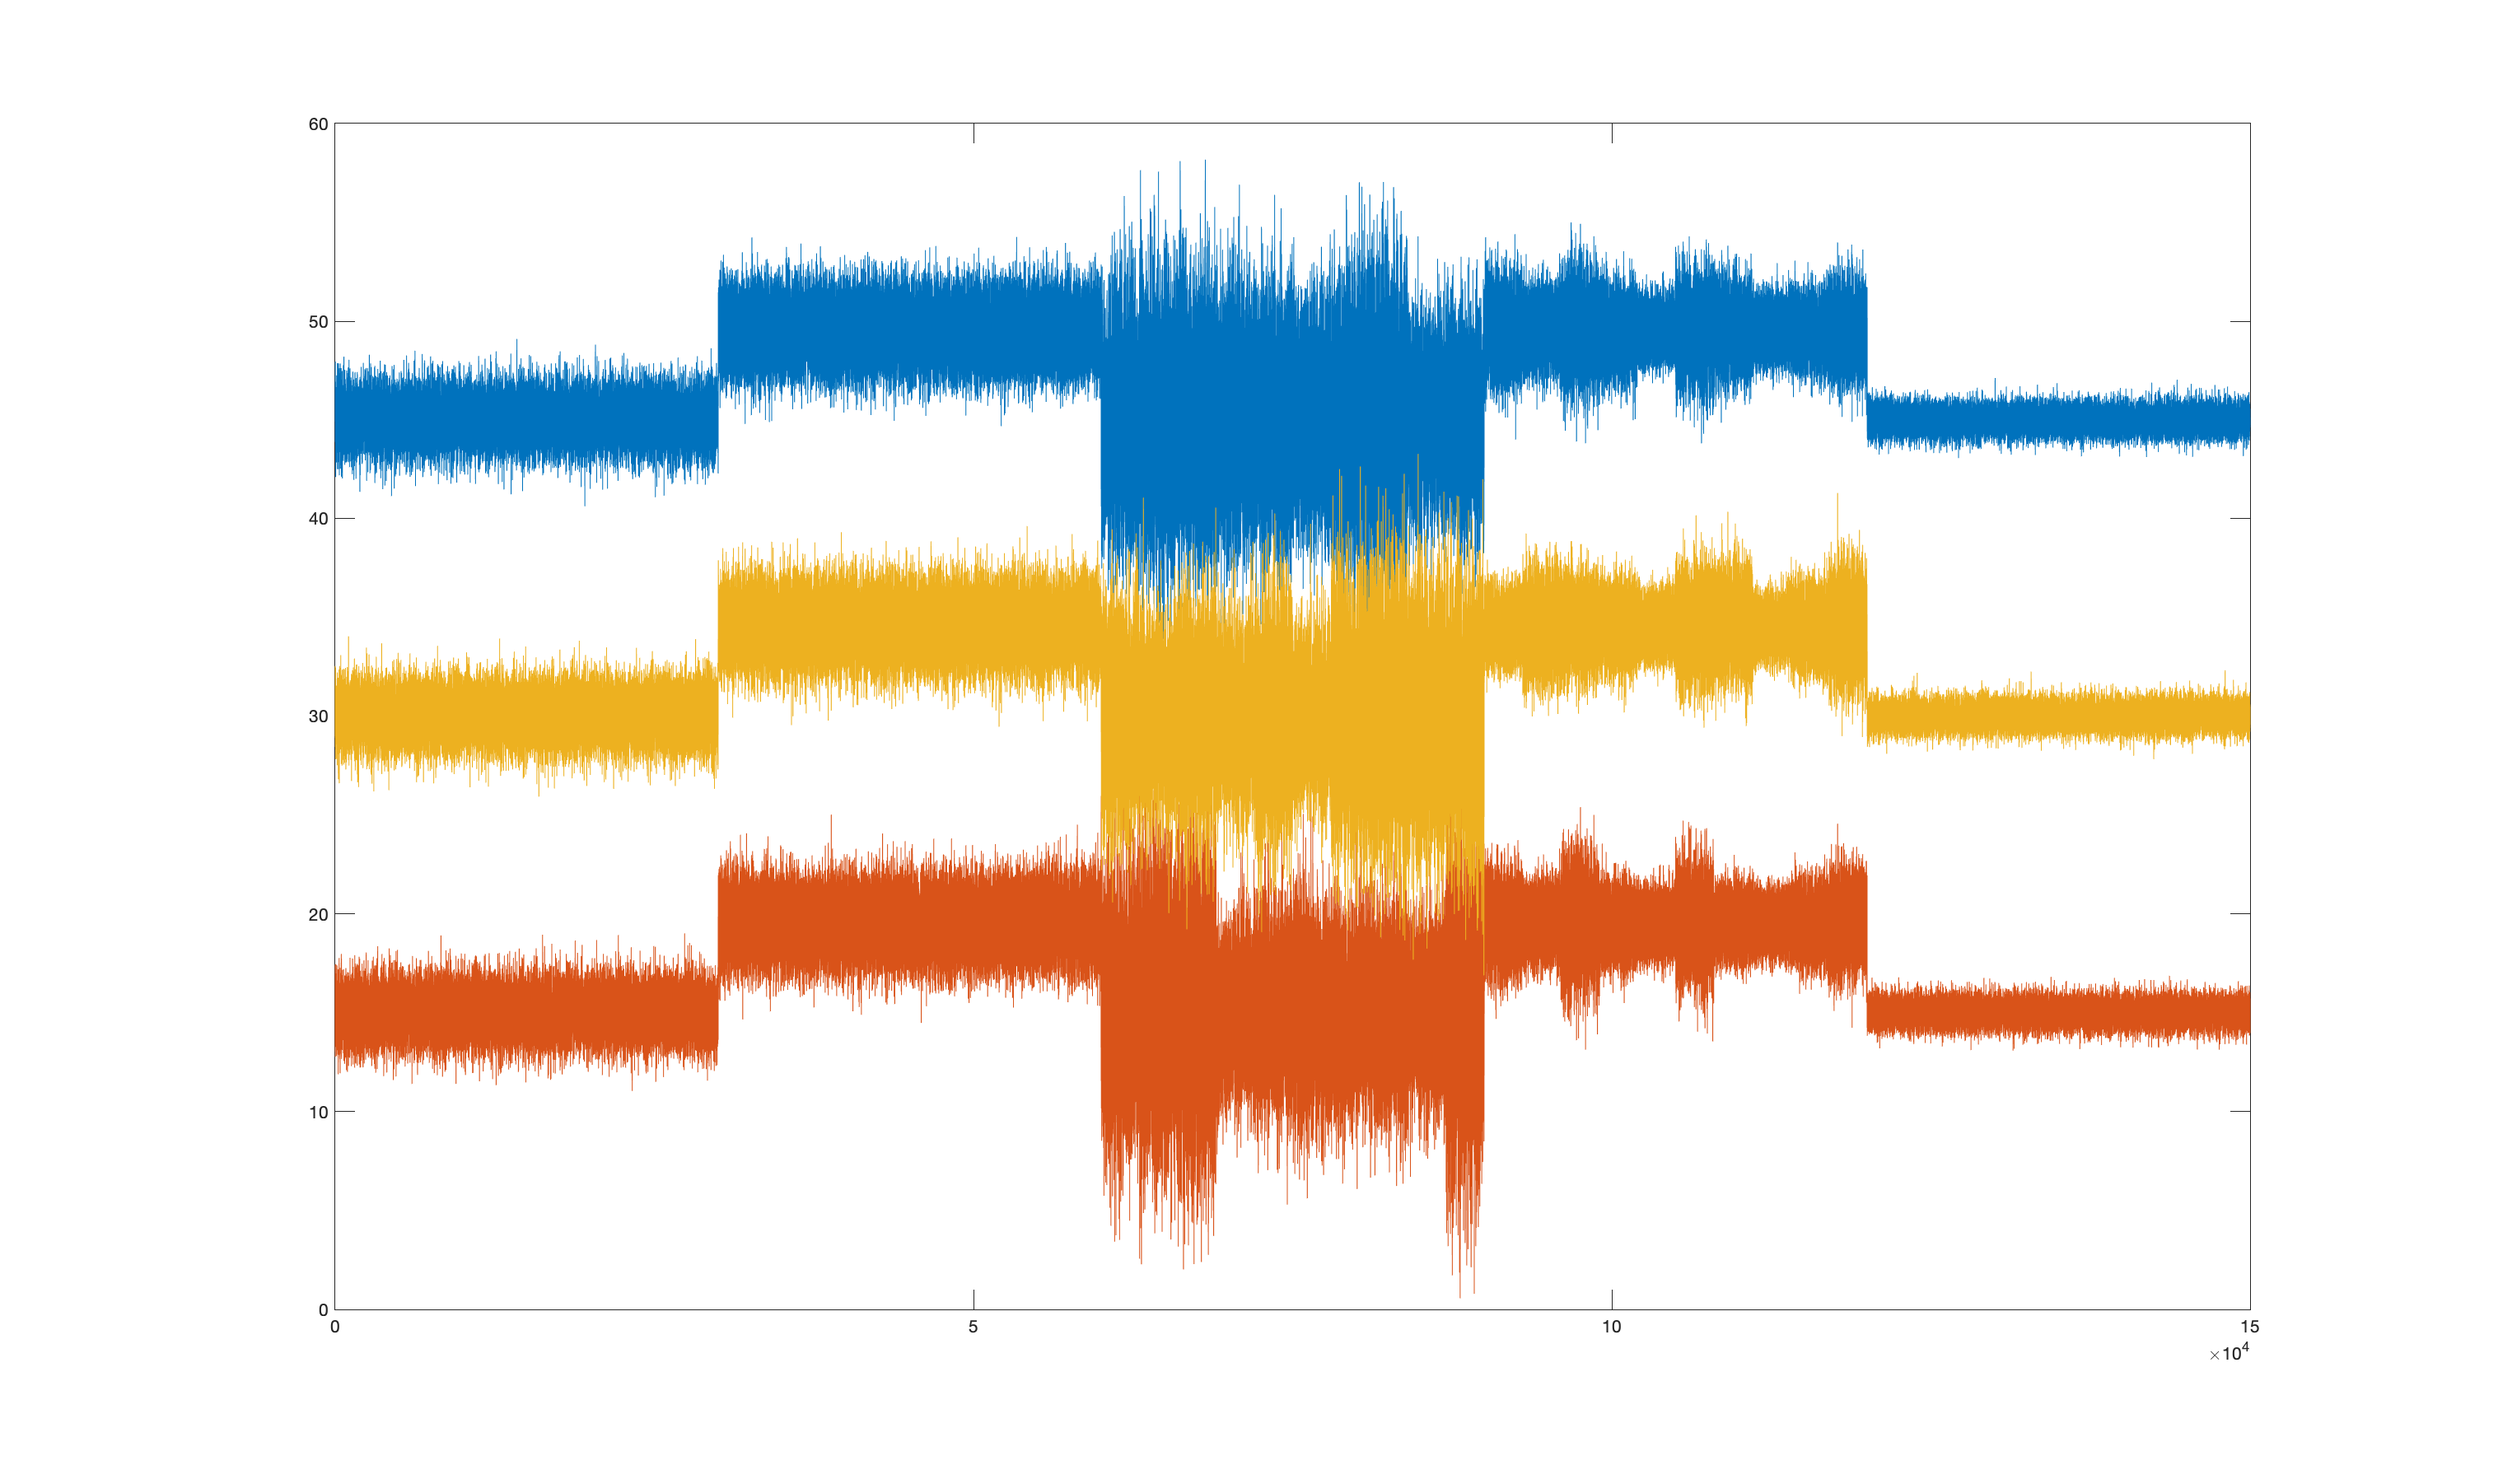
\includegraphics[width=3cm]{fig/Coriginal.eps} \\
        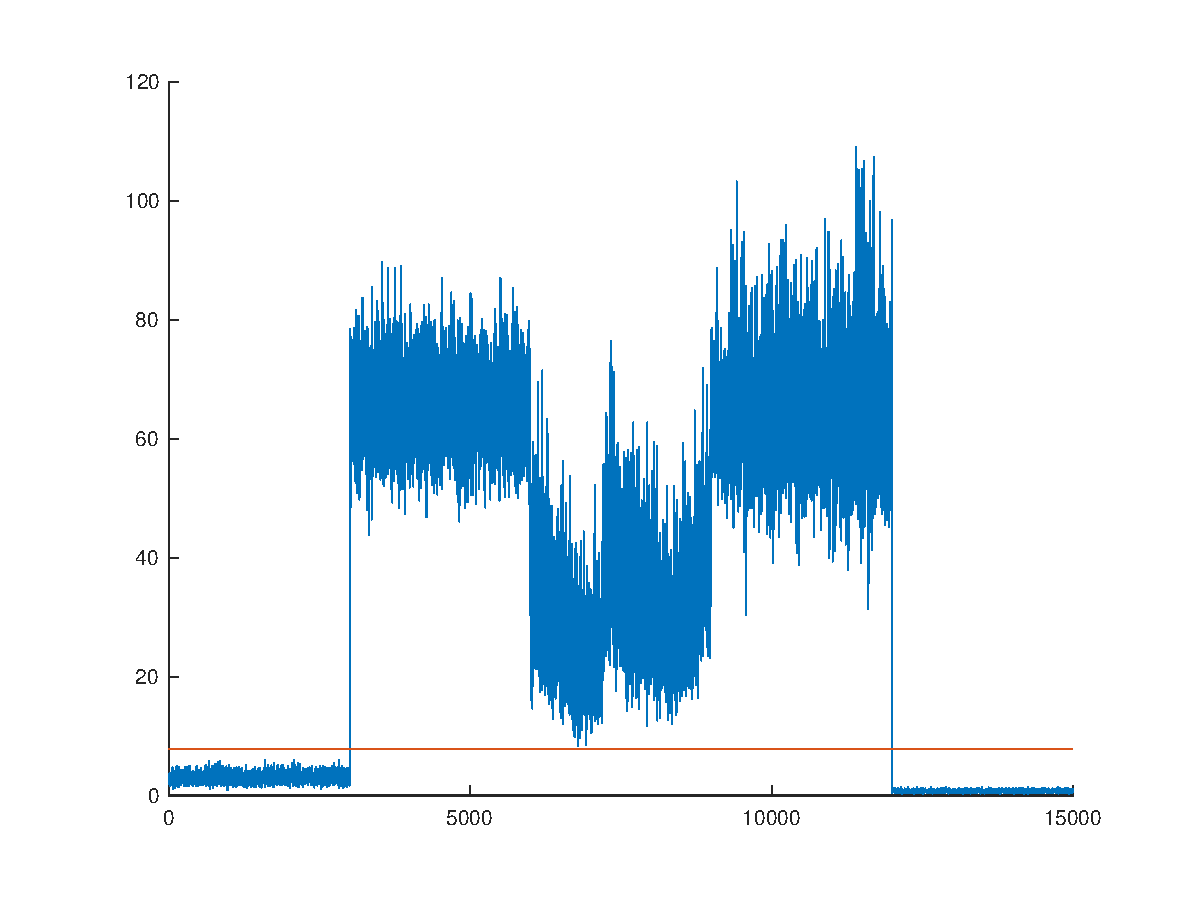
\includegraphics[width=3cm]{fig/thresholdT.eps} \\
        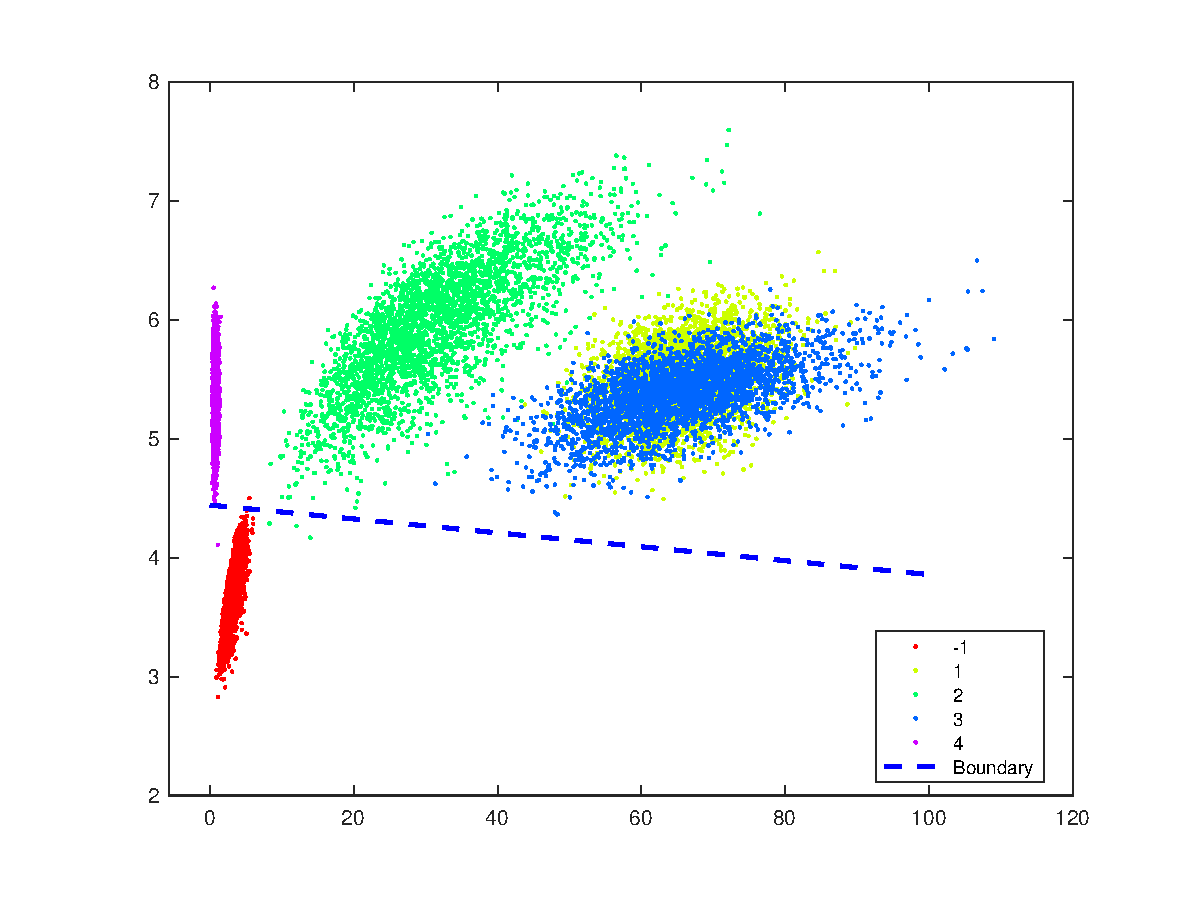
\includegraphics[width=3cm]{fig/miniVarP.eps}
        \end{figure}
    \end{frame}
    
    
    \begin{frame}{Case study on a numerical example}
    \begin{columns}
             \begin{column}{0.5\textwidth}
 \begin{small}
\begin{equation} \nonumber
\begin{aligned}
& w^Tx+b=0  \\
& D=sgn(w^Tx_i+b) = \left\{ 
    \begin{aligned}
  & -1  \\
  &\quad 1 
  \end{aligned}
     \right.
\end{aligned}
\end{equation}
\end{small}
 Case 1: \par  $\small{w^T = [ 0.4106 \quad -0.6689]
 , b = -3.473} $\par $\small{\alpha \approx 0.047\%,\beta  \approx  99.9\%,VA \approx 99.93\%}$ \par 
Case 2:  \par $\small{w^T = [0.3305 \quad -0.7488]
 , b = -0.8336} $\par $\small{\alpha \approx 0.33\%  ,\beta  \approx  98.8 \%,VA \approx 89.83 \%}$ \par
 where VA is validation accuracy.
           \end{column}
        \begin{column}{0.5\textwidth} 
         \begin{figure}
        \centering
        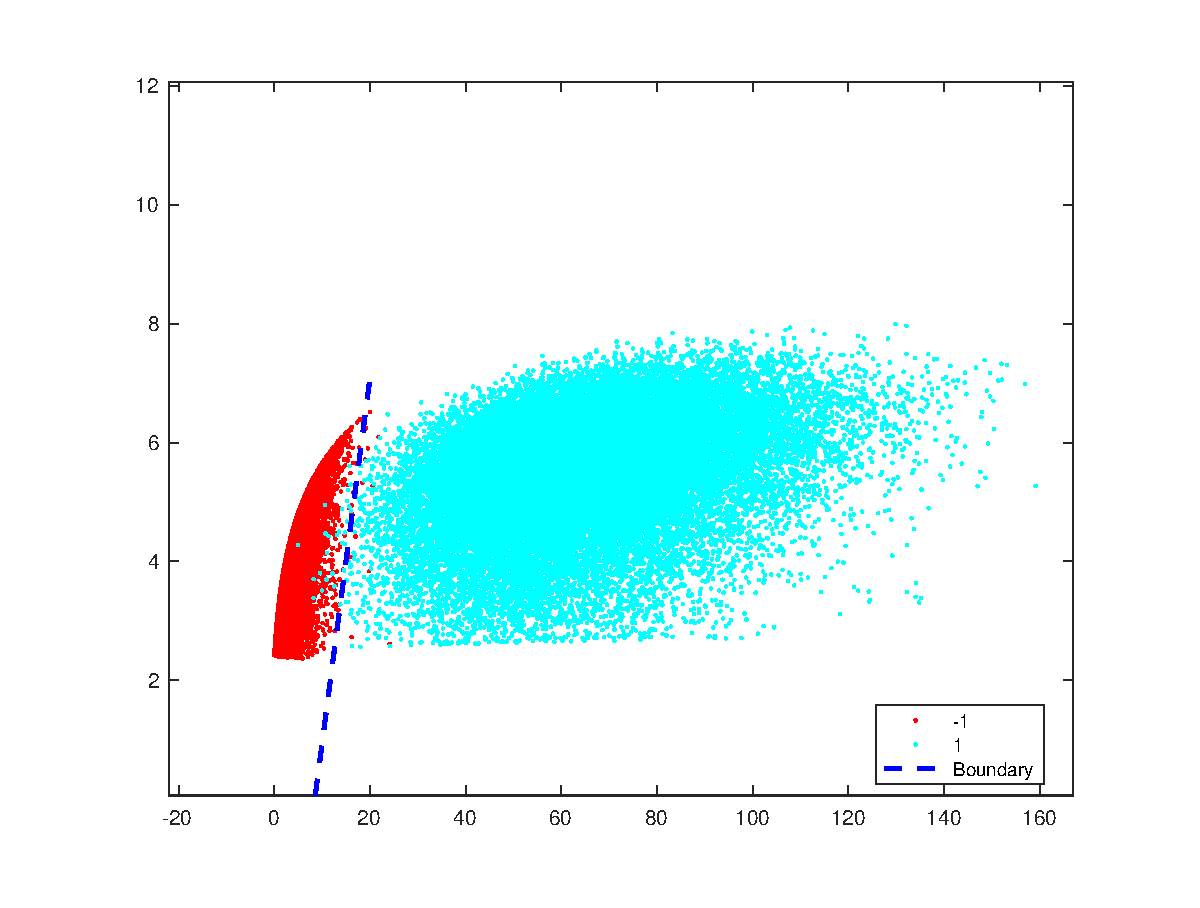
\includegraphics[width=4cm]{fig/addHyper.eps}
        \caption{$y_n$ and $y_a$ (case 1)}
        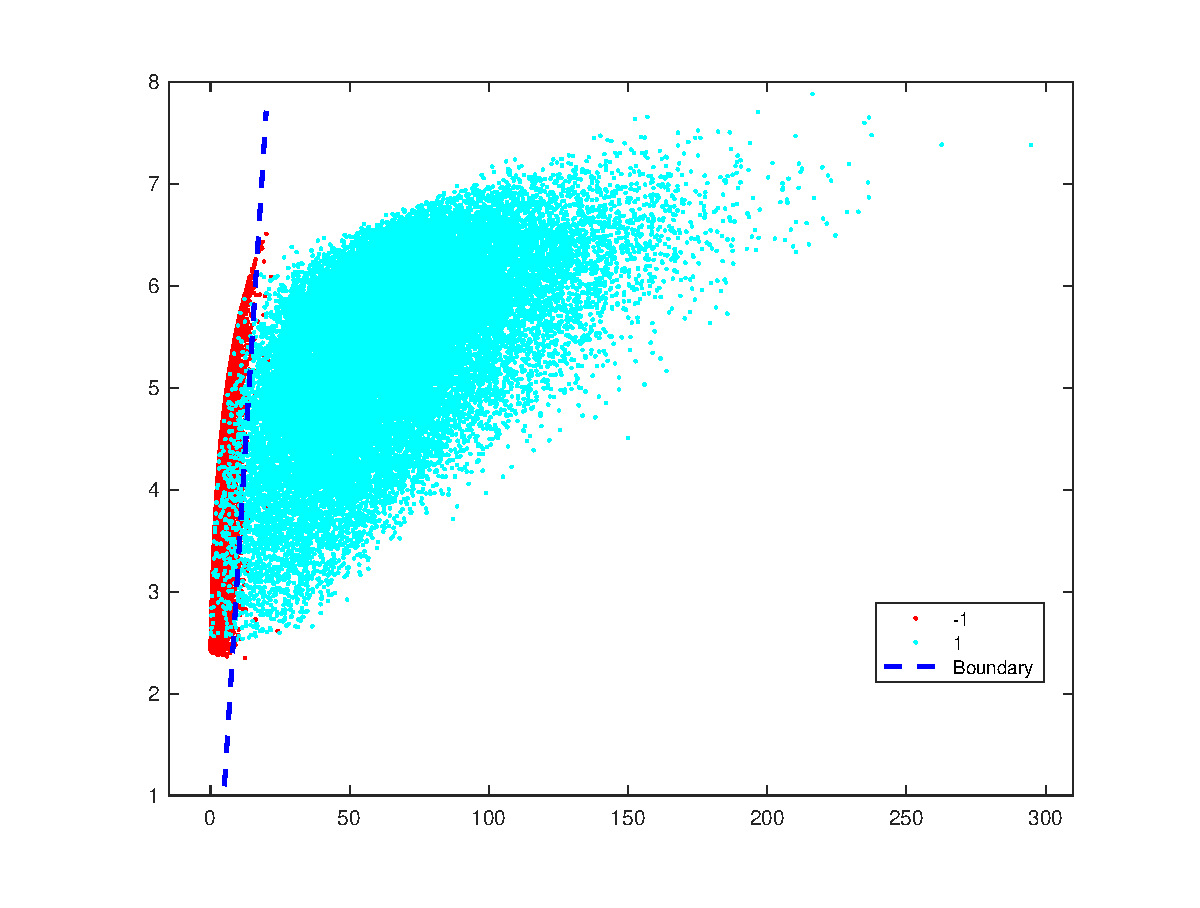
\includegraphics[width=4cm]{fig/ALhyperplane.eps}
        \caption{$y_n$ and $y_{am}$ (case 2)}
        \end{figure}
        \end{column}
    \end{columns}
\end{frame}

\begin{frame}{Case study on a numerical example}
     \begin{columns}
             \begin{column}{0.5\textwidth}
       Case 4: \par
     $\scriptsize{w^T = [ 0.8847 \quad 0.0007]
 , b =-6.3180 } $\par $\scriptsize{\alpha  \approx 0\%,\beta  \approx 99.99 \% ,VA \approx 99.99} \% $ \par 
Case 5: \par 
   $\scriptsize{w^T = [0.0481 \quad 5.2780]
 , b = -23.5837} $\par $\scriptsize{\alpha  \approx 3.3333\times 10^{-3} \%,\beta  \approx 99.97\% }$ \par 
$VA \approx 99.99 \% $
           \end{column}
        \begin{column}{0.5\textwidth}  %%<--- here
    \begin{figure}
        \centering
        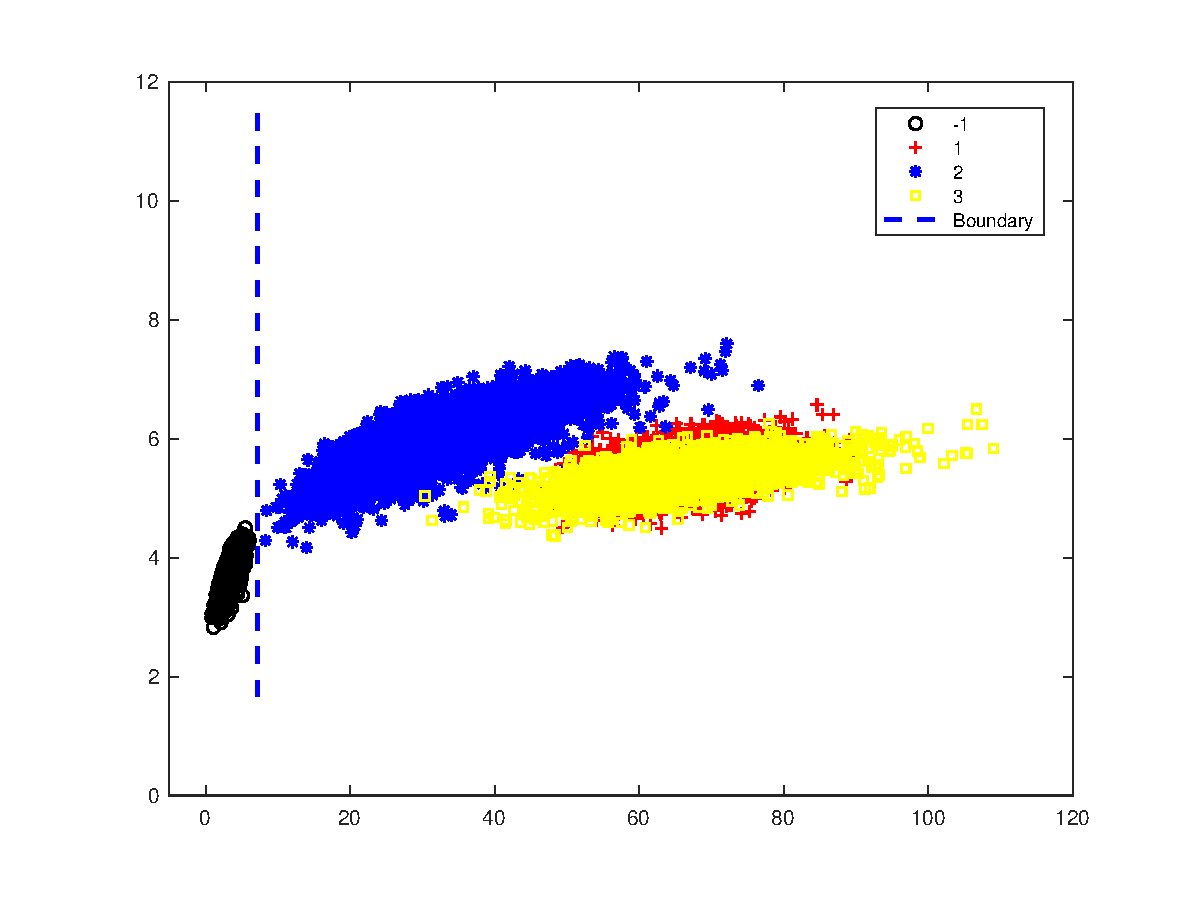
\includegraphics[width=4cm]{fig/Cu3.eps}
        \caption{$y_n,y_a,y_m,y_{am}$ (case 4)}
        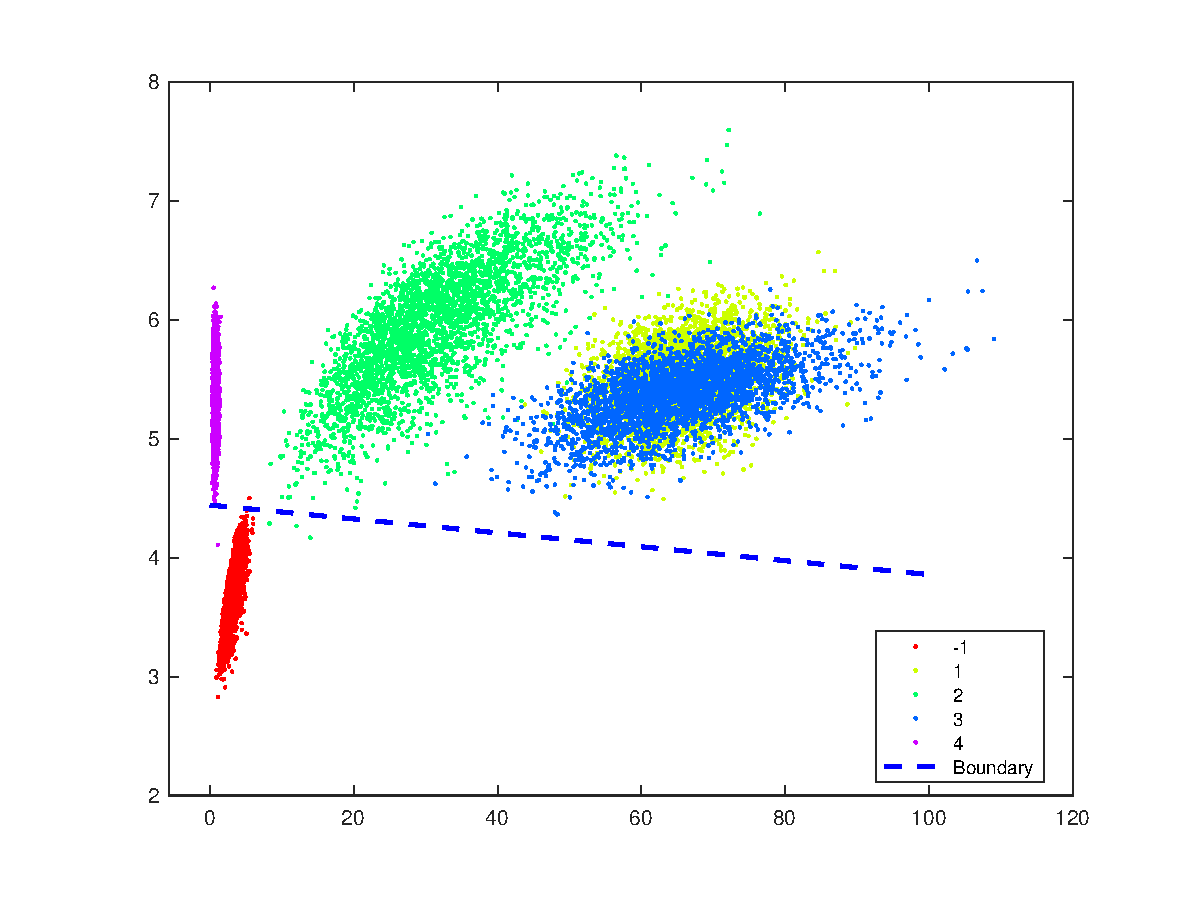
\includegraphics[width=4cm]{fig/miniVarP.eps}
        \caption{ $y_n,y_a,y_{m},y_{am},y_{ms}$ (case 5)}
        \end{figure}
  
        \end{column}
    \end{columns}
\end{frame}

\begin{frame}{Case study on a numerical example}
 \begin{columns}
             \begin{column}{0.5\textwidth}
   Case 3: \par
     $\small{w^T = [0.2859 \quad -0.1169]
 , b =-1.7315 } $\par $\small{\alpha  \approx 4.7\%,\beta  \approx 95 \% ,VA \approx}90.11 \% $ \par 
 With reference to the values of $\alpha$ and $\beta$, the prediction accuracy is satisfactory.
           \end{column}
        \begin{column}{0.4\textwidth}  %%<--- here
   \begin{figure}
        \centering
        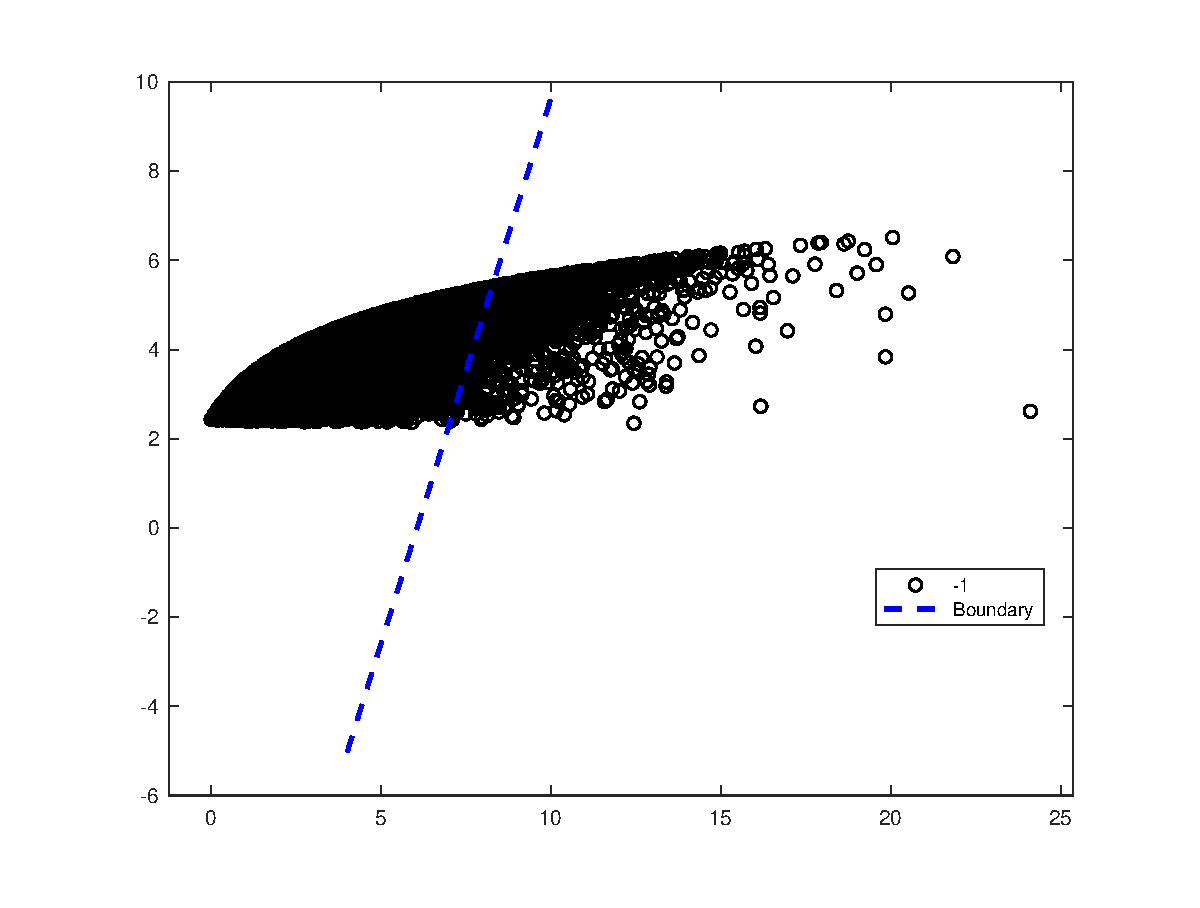
\includegraphics[width=4cm]{fig/EAandhyper.eps}
        \caption{$y_n$ data(case 3)}
        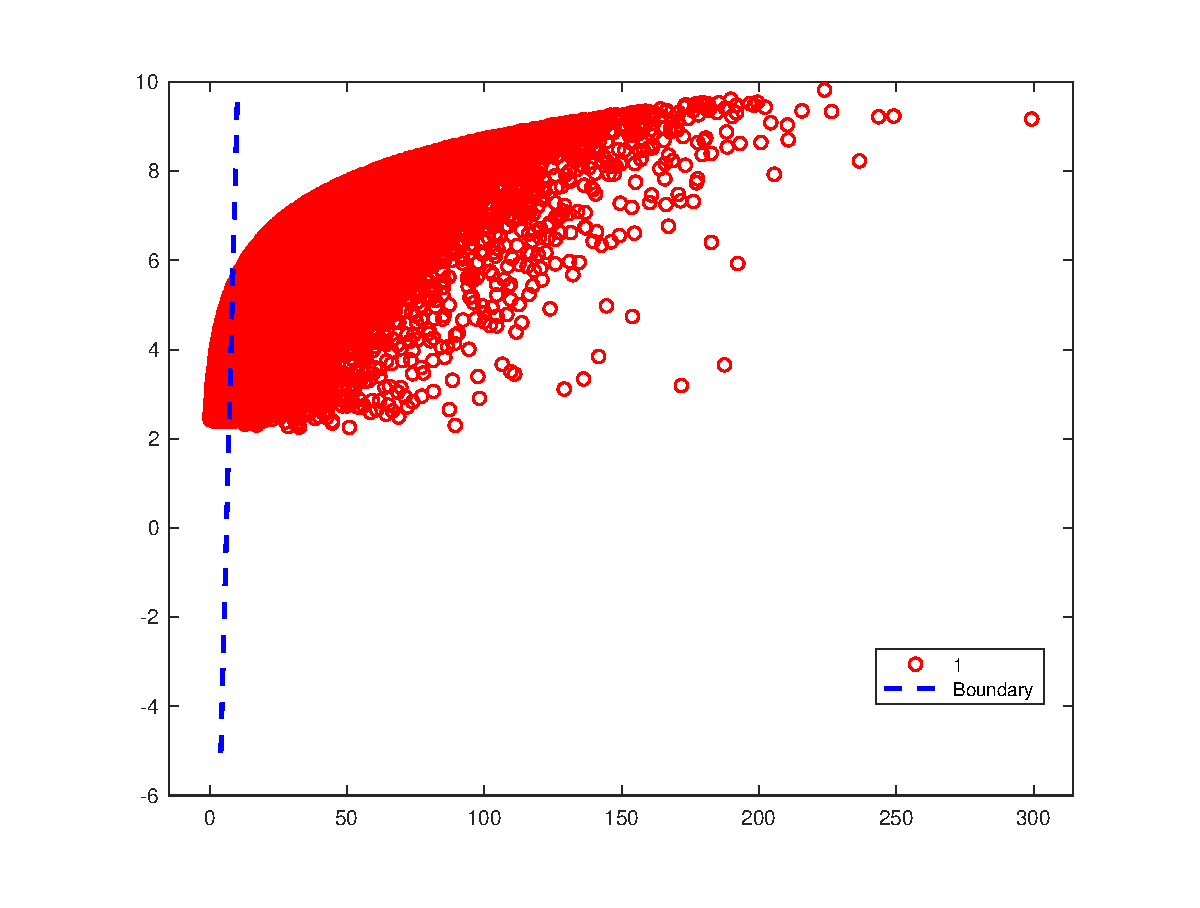
\includegraphics[width=4cm]{fig/EMandhyper.eps}
        \caption{ $y_{m}$ data(case 3)}
        \end{figure}
        \end{column}
    \end{columns}    
\end{frame}
\begin{frame}{Case study on a numerical example}
     \metroset{block=fill}
      \begin{exampleblock}{Data reoptimization}
	\begin{itemize}
    \item Cumulative  $T^2$-statistic
    \item Cumulative  Riemannian metric
    \end{itemize}
    \end{exampleblock}
    \begin{small}
    \begin{equation}\nonumber
       \begin{aligned}
       J_{T_n^2}(j) = \frac{1}{n}\sum_{i}^{i+n-1}J_{T^2}(i) \\
       J_{R_n}(j) = \frac{1}{n}\sum_{i}^{i+n-1}J_R(i)
       \end{aligned}
    \end{equation}
    \end{small}
\end{frame}
\begin{frame}
\frametitle{Riemannian distance as evaluation function}
    \textbf{How to get data matrices on Riemannian manifold?}\\
 Suppose we have a data batch $A \in \mathbb{R}^{M \times N}$, we can get $N-w$ data matrices on the Riemannian manifold by 
 \begin{equation}
    \begin{split}
    \hat{Y_i} &=\frac{1}{w+1} 
    \begin{bmatrix}
    A(:,i) & A(:,i+1) & \cdots & A(:,i+w)
    \end{bmatrix}
    \begin{bmatrix}
        A(:,i)^T \\ A(:,i+1)^T \\ \vdots \\ A(:,i+w)^T
    \end{bmatrix},\\
    Y_i &= \hat{Y_i}  + diag(0.0001,\cdots, 0.0001), Y_i \in \mathbb{R}^{M \times M} ,\  i = 1,\cdots , N-w.
 \label{eq:SPD}
\end{split}
 \end{equation}
Then $Y_i$ is symmetric positive definite(SPD).

      \begin{equation}
              S_i = y_iy_i^T+diag(d_1 \dots d_m)
    \end{equation}
\end{frame}
\end{document}
